\documentclass[10pt,a4paper]{article}

% ============================================================
%  Seminararbeit - Effiziente Programmierung (C/C++)
%  Thema 16: Ueberladen von Operatoren
%  Hochschule Mainz - Fachbereich Technik
% ============================================================

% ---------- Encoding ----------
\usepackage[utf8]{inputenc}
\usepackage[T1]{fontenc}

% ---------- Page geometry ----------
\usepackage[a4paper,left=2.5cm,right=2.5cm,top=2.3cm,bottom=2.3cm]{geometry}

% ---------- Line spacing ----------
\usepackage{setspace}
\setstretch{1.23}
\setlength{\emergencystretch}{2em}
\setlength{\textfloatsep}{8pt plus 2pt minus 2pt}
\setlength{\intextsep}{8pt plus 2pt minus 2pt}
\setlength{\abovecaptionskip}{6pt}
\setlength{\belowcaptionskip}{2pt}

% ---------- Graphics, color, tables ----------
\usepackage{graphicx}
\usepackage{xcolor}
\usepackage{booktabs}
\usepackage{array}
\usepackage{multirow}
\usepackage{float}
\usepackage[section]{placeins}

% ---------- Hochschule Mainz green ----------
\definecolor{hsmgreen}{RGB}{157,191,53}

% ---------- Math ----------
\usepackage{amsmath}
\usepackage{amssymb}

% ---------- German section labels (no babel available) ----------
\renewcommand{\contentsname}{Inhaltsverzeichnis}
\renewcommand{\listfigurename}{Abbildungsverzeichnis}
\renewcommand{\listtablename}{Tabellenverzeichnis}
\renewcommand{\figurename}{Abbildung}
\renewcommand{\tablename}{Tabelle}
\renewcommand{\refname}{Quellenverzeichnis}
\renewcommand{\appendixname}{Anhang}

% ---------- Code listings ----------
\usepackage{listings}
\lstset{
  language=C++,
  basicstyle=\ttfamily\small,
  keywordstyle=\color{blue!70!black}\bfseries,
  commentstyle=\color{green!50!black}\itshape,
  stringstyle=\color{orange!80!black},
  numbers=left,
  numberstyle=\tiny\color{gray},
  stepnumber=1,
  numbersep=8pt,
  showstringspaces=false,
  breaklines=true,
  frame=single,
  rulecolor=\color{gray!40},
  backgroundcolor=\color{gray!5},
  captionpos=b,
  tabsize=2,
  xleftmargin=15pt,
  literate={ä}{{\"a}}1 {ö}{{\"o}}1 {ü}{{\"u}}1 {Ä}{{\"A}}1 {Ö}{{\"O}}1 {Ü}{{\"U}}1 {ß}{{\ss}}1 {✓}{{$\checkmark$}}1 {✗}{{$\times$}}1 {×}{{$\times$}}1 {³}{{$^3$}}1 {Δ}{{$\Delta$}}1
}

% ---------- Headers & footers ----------
\usepackage{fancyhdr}
\pagestyle{fancy}
\fancyhf{}
\fancyhead[L]{\small Überladen von Operatoren}
\fancyhead[R]{\small Effiziente Programmierung (C/C++)}
\fancyfoot[C]{\thepage}
\renewcommand{\headrulewidth}{0.4pt}
\setlength{\headheight}{14pt}

% ---------- Captions ----------
\usepackage[font=small,labelfont=bf]{caption}

% ---------- Hyperlinks ----------
\usepackage[hidelinks,hypertexnames=false]{hyperref}

% ============================================================
\begin{document}

% ============================================================
%  DECKBLATT
% ============================================================
\begin{titlepage}
\begin{center}

\vspace*{0.5cm}

% --- Logo ---
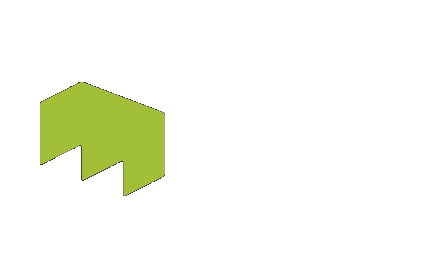
\includegraphics[width=0.45\textwidth]{hsm_logo.png}

\vspace{1.5cm}

{\Large Hochschule Mainz}\\[0.2cm]
{\large Fachbereich Technik}\\[0.2cm]
{\large Studiengang [Ihr Studiengang]}

\vspace{2.0cm}

% --- Colored rule ---
{\color{hsmgreen}\rule{\textwidth}{2pt}}

\vspace{0.8cm}

{\Huge\bfseries Überladen von Operatoren in C++}\\[0.5cm]
{\Large Konzepte, Implementierung und Effizienzanalyse}

\vspace{0.8cm}

{\color{hsmgreen}\rule{\textwidth}{2pt}}

\vspace{1.5cm}

{\large Seminararbeit\\[0.2cm]
im Modul \textbf{Effiziente Programmierung (C/C++)}\\[0.2cm]
Thema 16}

\vspace{2.0cm}

\begin{tabular}{rl}
\textbf{Vorgelegt von:} & [Vor- und Nachname]\\[0.2cm]
\textbf{Matrikelnummer:} & [Matrikelnummer]\\[0.2cm]
\textbf{E-Mail:} & [E-Mail-Adresse]\\[0.6cm]
\textbf{Betreuung:} & Jessica Buchner\\[0.6cm]
\textbf{Abgabedatum:} & 14.06.2026\\
\end{tabular}

\vfill

\end{center}
\end{titlepage}

% ============================================================
%  INHALTSVERZEICHNIS
% ============================================================
\pagenumbering{Roman}
\tableofcontents
\newpage

% ============================================================
%  HAUPTTEXT
% ============================================================
\pagenumbering{arabic}
\setcounter{page}{1}

% ------------------------------------------------------------
\section{Einleitung}
\label{sec:einleitung}

\subsection{Motivation und Problemstellung}

Das Überladen von Operatoren gehört zu den charakteristischen Sprachmerkmalen
von C++. Es erlaubt es, die in der Sprache vordefinierten Operatoren wie
\texttt{+}, \texttt{-}, \texttt{*}, \texttt{==} oder \texttt{[]} auch auf
selbst definierte Datentypen anzuwenden. Statt eine Addition zweier Matrizen
über einen Methodenaufruf wie \texttt{A.add(B)} auszudrücken, kann eine
benutzerdefinierte Klasse so gestaltet werden, dass der intuitive Ausdruck
\texttt{A + B} möglich wird. Auf diese Weise verhalten sich eigene Typen
syntaktisch wie eingebaute Typen, was die Lesbarkeit und Ausdrucksstärke des
Quellcodes erhöht \cite{stroustrup2013,cppreference}.

Diese syntaktische Eleganz ist jedoch nicht kostenlos. Hinter einem schlicht
aussehenden Ausdruck wie \texttt{D = A + B + C} können sich zahlreiche
implizite Operationen verbergen: die Erzeugung temporärer Objekte, das
Kopieren großer Datenmengen sowie wiederholte Speicheranforderungen auf dem
Heap. Gerade weil diese Kosten im Quelltext nicht unmittelbar sichtbar sind,
besteht die Gefahr, dass ineffizienter Code entsteht, ohne dass dies dem
Entwickler bewusst wird. Im Kontext der effizienten Programmierung ist die
Operatorüberladung somit ein anschauliches Beispiel dafür, dass lesbarer Code
und performanter Code nicht zwangsläufig identisch sind, sich durch geeignete
Implementierungstechniken aber miteinander vereinbaren lassen.

Zentral für diese Vereinbarkeit sind moderne C++-Konzepte wie die
Move-Semantik, rvalue-Referenzen sowie compilerseitige Optimierungen wie die
Return Value Optimization (RVO). Sie ermöglichen es, die durch
Operatorüberladung entstehenden temporären Objekte zu vermeiden oder
kostengünstig zu verschieben, anstatt sie aufwändig zu kopieren. Welchen
konkreten Einfluss unterschiedliche Implementierungsvarianten auf Laufzeit,
Speicherverbrauch und die Anzahl temporärer Objekte haben, bildet den Kern
der vorliegenden Untersuchung.

Für die Einordnung der Messergebnisse ist dabei ein Standarddetail zentral:
Seit C++17 wird bei der Initialisierung eines neuen Objekts aus einem
prvalue -- etwa in \texttt{Matrix D = A + B;} -- der Rückgabewert
verpflichtend ohne zusätzliche Kopie oder Move materialisiert
("guaranteed copy elision"). Dadurch unterscheiden sich naive und
move-fähige Implementierungen in genau diesem Fall oft kaum, selbst bei
\texttt{-O0}. Relevante Unterschiede durch Move-Semantik zeigen sich vor
allem bei der Zuweisung aus Temporaries (z.\,B. \texttt{C = A + B;}), bei
verketteten Ausdrücken mit echten Zwischenwerten (z.\,B.
\texttt{A + B + C}) und bei Container-Reallokationen \cite{cppreference_elision,meyers2014}.

\subsection{Zielsetzung}

Ziel dieser Arbeit ist es, das Überladen von Operatoren in C++ sowohl
theoretisch fundiert darzustellen als auch dessen Effizienzaspekte empirisch
zu untersuchen. Anhand einer beispielhaften Klasse werden mehrere
Implementierungsvarianten desselben Operators entwickelt und systematisch
miteinander verglichen. Im Mittelpunkt stehen dabei die folgenden Fragen:
Wie wirken sich die naive Implementierung, die Nutzung der Move-Semantik
sowie eine auf zusammengesetzten Zuweisungsoperatoren basierende Variante auf
die Performance aus? Welche Rolle spielen dabei die Optimierungsstufen des
Compilers? Und in welchem Umfang lassen sich temporäre Objekte durch geeignete
Techniken tatsächlich einsparen? Die Arbeit verfolgt damit das Ziel, ein
fundiertes Verständnis für die Effizienzimplikationen der Operatorüberladung
zu vermitteln und daraus praktische Empfehlungen abzuleiten.

\subsection{Aufbau der Arbeit}

Die Arbeit gliedert sich in vier Hauptteile. Kapitel~\ref{sec:theorie} legt
die theoretischen Grundlagen der Operatorüberladung dar und behandelt unter
anderem die Unterscheidung zwischen Member- und Nicht-Member-Funktionen, die
Rule of Three/Five/Zero sowie die Move-Semantik. Kapitel~\ref{sec:implementierung}
beschreibt die praktische Umsetzung der verschiedenen Implementierungsvarianten
einschließlich einer Instrumentierung zur Zählung temporärer Objekte.
Kapitel~\ref{sec:experimente} stellt den Versuchsaufbau vor und präsentiert
sowie interpretiert die Messergebnisse hinsichtlich Laufzeit, Speicherverbrauch
und temporärer Objekte. Kapitel~\ref{sec:fazit} fasst die Erkenntnisse
zusammen und gibt Empfehlungen für den praktischen Einsatz der
Operatorüberladung.

% ------------------------------------------------------------
\section{Theoretischer Hintergrund}
\label{sec:theorie}

\subsection{Grundlagen der Operatorüberladung}
In C++ ist ein Operator im Kern nichts anderes als eine Funktion mit einer besonderen, vom Compiler erkannten Schreibweise. Wenn der Compiler einen Ausdruck wie \texttt{a + b} verarbeitet, übersetzt er ihn intern in einen Funktionsaufruf -- entweder \texttt{a.operator+(b)}, falls der Operator als Member-Funktion definiert ist, oder \texttt{operator+(a, b)}, falls er als freie Funktion vorliegt. Das Überladen von Operatoren bedeutet daher lediglich, für einen oder beide Operanden eines benutzerdefinierten Typs eine solche \texttt{operator}-Funktion bereitzustellen. Die Syntax folgt dem Schema \texttt{Rückgabetyp operator<symbol>(Parameter)}, wobei \texttt{<symbol>} für den jeweiligen Operator steht, etwa \texttt{+}, \texttt{==} oder \texttt{[]}.

Diese Grundlagen und die zugehörigen Sprachregeln sind in der Standardliteratur sowie in der Referenzdokumentation umfassend beschrieben \cite{stroustrup2013,cppreference}.

Wichtig ist, dass mindestens ein Operand ein benutzerdefinierter Typ (also eine Klasse, Struktur oder ein Enum) sein muss. Es ist nicht möglich, das Verhalten von Operatoren für ausschließlich eingebaute Typen zu verändern -- ein Ausdruck wie \texttt{1 + 2} lässt sich nicht umdefinieren. Diese Einschränkung verhindert, dass die fundamentale Semantik der Sprache durch eigene Definitionen unterlaufen wird.

Nicht jeder Operator kann überladen werden. Die überwiegende Mehrheit ist überladbar, darunter die arithmetischen Operatoren (\texttt{+}, \texttt{-}, \texttt{*}, \texttt{/}, \texttt{\%}), die Vergleichsoperatoren (\texttt{==}, \texttt{!=}, \texttt{<}, \texttt{>}, \texttt{<=}, \texttt{>=}), die logischen Operatoren, der Indexzugriff \texttt{[]}, der Funktionsaufrufoperator \texttt{()}, der Dereferenzierungsoperator \texttt{*} und der Pfeiloperator \texttt{->}, die Zuweisungsoperatoren sowie die Stream-Operatoren \texttt{<<} und \texttt{>>}. Einige wenige Operatoren sind hingegen ausdrücklich von der Überladung ausgeschlossen: der Bereichsauflösungsoperator \texttt{::}, der Member-Zugriff über Punkt \texttt{.}, der Member-Pointer-Zugriff \texttt{.*}, der ternäre Bedingungsoperator \texttt{?:} sowie \texttt{sizeof} und \texttt{typeid}. Der Grund liegt darin, dass diese Operatoren auf einer so grundlegenden Ebene der Sprache arbeiten, dass eine Umdefinition zu nicht auflösbaren Mehrdeutigkeiten oder zum Verlust der Typsicherheit führen würde.

Bei der Überladung gibt es eine zentrale Regel, die zwar nicht vom Compiler erzwungen, in der Praxis aber als verbindlich gilt: Ein überladener Operator sollte sich semantisch so verhalten, wie es von ihm intuitiv erwartet wird. Ein \texttt{operator+} sollte etwas addieren oder zusammenfügen und keine Seiteneffekte auslösen, die den Zustand der Operanden verändern. Wird diese Konvention verletzt -- etwa indem \texttt{operator+} in Wahrheit eine Subtraktion durchführt -- bleibt der Code zwar lauffähig, wird aber unleserlich und fehleranfällig. Die Stärke der Operatorüberladung liegt gerade darin, dass eigene Typen sich erwartungskonform verhalten; diese Erwartungskonformität ist Voraussetzung für ihren sinnvollen Einsatz.

Ein weiterer grundlegender Aspekt betrifft die Frage, was ein Operator zurückgeben sollte. Hier hat sich eine Konvention etabliert, die eng mit der Effizienz zusammenhängt und die in Kapitel~4 empirisch untersucht wird: Operatoren, die ein neues Objekt erzeugen (wie \texttt{operator+}), geben üblicherweise per Wert zurück, da das Ergebnis ein eigenständiges, neues Objekt ist. Operatoren hingegen, die einen bestehenden Operanden verändern (wie \texttt{operator+=}), geben üblicherweise eine Referenz auf diesen Operanden zurück, um Verkettungen wie \texttt{a += b += c} zu ermöglichen und unnötige Kopien zu vermeiden. Diese Unterscheidung zwischen Wert- und Referenzrückgabe ist nicht nur eine Stilfrage, sondern hat unmittelbare Auswirkungen auf die Anzahl der erzeugten temporären Objekte und damit auf die Performance.

\subsection{Member- vs. Nicht-Member-Funktionen}

Ein überladener Operator kann auf zwei Arten implementiert werden: als Member-Funktion der Klasse oder als freie (Nicht-Member-)Funktion außerhalb der Klasse. Beide Varianten sind funktional weitgehend gleichwertig, unterscheiden sich jedoch in wichtigen Details, die die Wahl im Einzelfall bestimmen.

Wird ein Operator als Member-Funktion definiert, so ist der linke Operand stets das Objekt, auf dem die Funktion aufgerufen wird (\texttt{*this}), während der rechte Operand als Parameter übergeben wird. Ein binärer Operator wie \texttt{+} benötigt als Member daher nur einen einzigen Parameter. Der Ausdruck \texttt{a + b} wird in diesem Fall zu \texttt{a.operator+(b)} übersetzt. Der entscheidende Vorteil der Member-Variante ist der direkte Zugriff auf die privaten Datenmember der Klasse, ohne dass eine zusätzliche \texttt{friend}-Deklaration nötig wäre.

Wird der Operator hingegen als freie Funktion definiert, so werden beide Operanden als explizite Parameter übergeben. Ein binärer Operator benötigt in dieser Form zwei Parameter, und der Ausdruck \texttt{a + b} wird zu \texttt{operator+(a, b)}. Da eine freie Funktion außerhalb der Klasse steht, hat sie standardmäßig keinen Zugriff auf deren private Member. Benötigt sie diesen Zugriff, muss sie innerhalb der Klasse als \texttt{friend} deklariert werden, oder die Klasse muss öffentliche Zugriffsmethoden bereitstellen.

Die Wahl zwischen beiden Formen folgt einigen etablierten Faustregeln. Operatoren, die den linken Operanden zwingend verändern und untrennbar mit dem Objekt verbunden sind, werden in der Regel als Member implementiert. Dazu gehören insbesondere die zusammengesetzten Zuweisungsoperatoren wie \texttt{+=} und \texttt{-=}. Für den Zuweisungsoperator \texttt{=}, den Indexoperator \texttt{[]}, den Funktionsaufrufoperator \texttt{()} sowie den Pfeiloperator \texttt{->} ist die Member-Form sogar zwingend vorgeschrieben.

Symmetrische binäre Operatoren wie \texttt{+}, \texttt{-}, \texttt{*} und insbesondere die Vergleichsoperatoren werden hingegen häufig als freie Funktionen bevorzugt. Der Grund dafür liegt in der Behandlung impliziter Typumwandlungen. Ist \texttt{operator+} als Member definiert, so wird der linke Operand bevorzugt behandelt: Eine implizite Umwandlung kann nur auf den als Parameter übergebenen rechten Operanden, nicht aber auf das aufrufende Objekt angewendet werden. Konkret bedeutet das: Existiert für eine Klasse \texttt{Number} ein Konstruktor, der aus einem \texttt{int} ein \texttt{Number}-Objekt erzeugt, so funktioniert bei der Member-Variante zwar der Ausdruck \texttt{n + 5} (der \texttt{int} wird in ein \texttt{Number} umgewandelt), nicht aber \texttt{5 + n}, da auf das linke Literal \texttt{5} keine Member-Funktion aufgerufen werden kann. Wird \texttt{operator+} hingegen als freie Funktion definiert, sind beide Operanden gleichberechtigt, und beide Ausdrücke -- \texttt{n + 5} ebenso wie \texttt{5 + n} -- lassen sich durch implizite Umwandlung auflösen. Diese Symmetrie ist der Hauptgrund, weshalb symmetrische arithmetische Operatoren und Vergleichsoperatoren konventionell als freie Funktionen implementiert werden.

Ein weiterer, häufig auftretender Fall sind die Stream-Operatoren \texttt{<<} und \texttt{>>}. Diese müssen zwingend als freie Funktionen implementiert werden, da ihr linker Operand ein Stream-Objekt (etwa \texttt{std::ostream}) ist und nicht der eigene benutzerdefinierte Typ. Eine Member-Implementierung würde voraussetzen, dass man die Klasse \texttt{std::ostream} selbst um eine Methode erweitern könnte, was nicht möglich ist. Da der Operator für eine korrekte Ausgabe in der Regel auf die internen Daten des eigenen Typs zugreifen muss, wird er üblicherweise als \texttt{friend} deklariert.

Eine in modernem C++ verbreitete Entwurfstechnik kombiniert beide Welten und ist zugleich für die Effizienzbetrachtung dieser Arbeit relevant: Der zusammengesetzte Operator \texttt{+=} wird als Member implementiert, da er den linken Operanden ohnehin verändert. Der symmetrische Operator \texttt{+} wird anschließend als freie Funktion definiert, die intern auf \texttt{+=} zurückgreift. Auf diese Weise wird die eigentliche Logik nur an einer Stelle gepflegt, Codeduplizierung vermieden und gleichzeitig die für symmetrische Operatoren wünschenswerte Behandlung beider Operanden gewährleistet. Diese Variante entspricht der in Kapitel~3 vorgestellten Version~3 und wird dort hinsichtlich ihrer Performance mit den übrigen Implementierungen verglichen.

Zusammenfassend lässt sich festhalten, dass die Entscheidung zwischen Member- und freier Funktion weniger eine Frage des persönlichen Stils als vielmehr eine Konsequenz aus der Semantik des jeweiligen Operators ist. Operatoren, die den linken Operanden verändern oder fest an ihn gebunden sind, gehören als Member in die Klasse; symmetrische Operatoren, die beide Operanden gleichberechtigt behandeln sollen, sind als freie Funktionen besser aufgehoben.

Diese Entwurfsprinzipien entsprechen etablierten Empfehlungen zur Operatorgestaltung in modernem C++ \cite{meyers2005,sutter2004,cppreference}.

\subsection{Spezielle Operatoren}

Einige Operatoren verdienen besondere Aufmerksamkeit, weil ihre Verwendung
häufig mit API-Design-Entscheidungen verknüpft ist. Der
Zuweisungsoperator \texttt{operator=} sollte Selbstzuweisung korrekt
behandeln und eine Referenz auf \texttt{*this} zurückgeben, damit
Verkettungen wie \texttt{a = b = c;} funktionieren. Der Indexoperator
\texttt{operator[]} wird in der Praxis meist in zwei Varianten angeboten,
als konstante und als nicht-konstante Überladung, damit sowohl lesender
als auch schreibender Zugriff effizient möglich ist.

Bei den Vergleichsoperatoren hat C++20 die Implementierung deutlich
vereinfacht: Mit dem Drei-Wege-Vergleich \texttt{operator<=>} kann die
totale Ordnung zentral beschrieben werden; daraus können klassische
Operatoren wie \texttt{<}, \texttt{<=}, \texttt{>} und \texttt{>=}
automatisch abgeleitet werden. Zusätzlich lassen sich
\texttt{operator==} und \texttt{operator<=>} häufig mit
\texttt{= default} deklarieren, wenn alle relevanten Member vergleichbar
sind. Das reduziert Boilerplate und verbessert die Konsistenz des
Vergleichsverhaltens.

Ein klassischer Sonderfall betrifft die logischen Operatoren \texttt{\&\&}
und \texttt{||}: Werden sie überladen, geht die eingebaute
Kurzschlussauswertung verloren. Beide Operanden werden dann ausgewertet,
was leicht zu unerwarteten Seiteneffekten und Performance-Nachteilen führt.
Deshalb werden diese Operatoren für benutzerdefinierte Typen nur in
Ausnahmefällen überladen.

\subsection{Rule of Three / Five / Zero}
Jede C++-Klasse verfügt über eine Reihe spezieller Elementfunktionen,
die der Compiler automatisch erzeugen kann: den Destruktor, den
Kopierkonstruktor, den Kopierzuweisungsoperator sowie -- seit C++11 --
den Move-Konstruktor und den Move-Zuweisungsoperator. Die sogenannten
``Rules'' sind Leitlinien dafür, wann ein Programmierer diese
Funktionen selbst definieren muss, anstatt sich auf die vom Compiler
erzeugten Varianten zu verlassen.

\paragraph{Rule of Three.}
Die Rule of Three besagt, dass eine Klasse, die einen benutzerdefinierten
Destruktor, Kopierkonstruktor oder Kopierzuweisungsoperator benötigt,
nahezu immer alle drei benötigt. Der Grund liegt in der
Ressourcenverwaltung. Eine Klasse, die eine rohe Ressource verwaltet --
typischerweise einen mit \texttt{new[]} angeforderten Speicherblock auf
dem Heap --, muss diesen in ihrem Destruktor wieder freigeben. Die vom
Compiler erzeugten Kopieroperationen führen jedoch eine flache Kopie
durch: Sie duplizieren den Zeiger, nicht den Speicherbereich, auf den er
verweist. Zwei Objekte verweisen dann auf denselben Block, was zu zwei
unabhängigen Destruktoraufrufen führt, die denselben Speicher
freigeben (\emph{double free}), sowie zu Aliasing, bei dem die Änderung
eines Objekts unbemerkt das andere verändert. Korrektes Verhalten
erfordert eine tiefe Kopie: das Anlegen eines neuen Speicherblocks und
das Kopieren der Elemente. Die Rule of Three koppelt die drei Funktionen
daher aneinander -- wer eine benötigt, benötigt alle \cite{meyers2005,sutter2004}.

\paragraph{Rule of Five.}
Mit C++11 wurde die Move-Semantik eingeführt und mit ihr zwei weitere
spezielle Elementfunktionen: der Move-Konstruktor und der
Move-Zuweisungsoperator. Die Rule of Five erweitert die Rule of Three um
diese beiden: Eine ressourcenverwaltende Klasse sollte alle fünf
Funktionen deklarieren. Über die bloße Symmetrie hinaus steht dahinter
ein subtiler, aber folgenreicher Grund. Der Compiler erzeugt für eine
Klasse, die einen Destruktor (oder eine Kopieroperation) deklariert,
keine Move-Operationen. Eine Klasse, die nur der Rule of Three folgt --
also einen Destruktor deklariert --, verliert somit stillschweigend ihre
Move-Operationen und fällt überall dort auf das Kopieren zurück, wo
ein Verschieben möglich gewesen wäre. Um die Effizienz der
Move-Semantik zurückzugewinnen, müssen Move-Konstruktor und
Move-Zuweisungsoperator explizit deklariert werden. Beide sollten als
\texttt{noexcept} gekennzeichnet sein: Standardcontainer wie
\texttt{std::vector} verschieben ihre Elemente bei einer Reallokation nur
dann, wenn der Move-Konstruktor \texttt{noexcept} ist; andernfalls
kopieren sie, um die starke Ausnahmegarantie zu wahren. Ein fehlendes
\texttt{noexcept} führt somit unbemerkt genau jene Kopien wieder ein,
die die Move-Semantik eigentlich vermeiden sollte \cite{meyers2014,coreguidelines}.

\paragraph{Rule of Zero.}
Die moderne Empfehlung besteht darin, manuelle Ressourcenverwaltung
gänzlich zu vermeiden. Speichert eine Klasse ihre Daten in Membern, die
ihre Ressourcen bereits selbst korrekt verwalten -- etwa
\texttt{std::vector}, \texttt{std::string} oder \texttt{std::unique\_ptr}
--, so sind die vom Compiler erzeugten speziellen Elementfunktionen
ihrerseits korrekt, und die Klasse sollte keine der fünf Funktionen
deklarieren. Eine Matrix, die einen \texttt{std::vector<double>} als
Speicher verwendet, folgt der Rule of Zero und erhält korrekte und
effiziente Kopier- und Move-Operationen kostenlos. Die in dieser Arbeit
untersuchten Implementierungen verwalten den Speicher bewusst manuell,
damit das Anlegen, Kopieren, Verschieben und Zerstören des
Speicherblocks beobachtbar und messbar wird; in produktivem Code wäre
die Rule of Zero der vorzuziehende Entwurf \cite{coreguidelines,meyers2014}.

\subsection{Kopier- und Move-Semantik}
Die Kopiersemantik beschreibt, was geschieht, wenn ein Objekt dupliziert
wird. Der Kopierkonstruktor erzeugt ein neues Objekt als eigenständige
Kopie eines bestehenden, während der Kopierzuweisungsoperator den Inhalt
eines bereits existierenden Objekts durch eine Kopie eines anderen
ersetzt. Für eine ressourcenverwaltende Matrix müssen beide eine tiefe
Kopie durchführen: einen neuen Speicherblock gleicher Größe anlegen
und jedes Element kopieren. Die Kosten sind daher proportional zur
Datenmenge -- eine Allokation zuzüglich eines elementweisen
Kopiervorgangs der Ordnung \(O(n)\) (bzw. \(O(n^2)\) für eine
\(n \times n\)-Matrix). Der Kopierzuweisungsoperator muss zusätzlich
den zuvor gehaltenen Speicher freigeben und sich gegen Selbstzuweisung
absichern.

Die Move-Semantik beschreibt, was geschieht, wenn die Eigentümerschaft an
einer Ressource übertragen statt dupliziert wird. Der Move-Konstruktor
und der Move-Zuweisungsoperator nehmen eine rvalue-Referenz
(\texttt{Matrix\&\&}) entgegen, die an temporäre Objekte bindet -- also
an Objekte, die ohnehin gleich zerstört werden und deren Ressourcen
daher gefahrlos ``gestohlen'' werden können. Anstatt zu allokieren und
zu kopieren, übernimmt ein Move-Vorgang lediglich Zeiger und Größe der
Quelle und versetzt diese in einen gültigen, leeren Zustand
(typischerweise Nullzeiger und Größe null), sodass ihr Destruktor keinen
Schaden anrichtet. Die Kosten sind konstant: einige wenige Zeiger- und
Ganzzahlzuweisungen, unabhängig von der Größe der Matrix. Es findet
weder eine Allokation noch ein elementweises Kopieren statt.

Der Mechanismus beruht auf den Wertkategorien (\emph{value categories}).
Ein lvalue besitzt einen Namen und eine dauerhafte Identität; ein rvalue
ist ein temporäres Objekt ohne bleibende Identität. Die
Move-Überladungen werden automatisch ausgewählt, wenn die Quelle ein
rvalue ist -- etwa das von \texttt{operator+} zurückgegebene temporäre
Objekt. Soll ein benanntes Objekt als verschiebbar behandelt werden,
kommt \texttt{std::move} zum Einsatz; diese Funktion verschiebt selbst
nichts, sondern stellt lediglich eine Umwandlung in eine rvalue-Referenz
dar, durch die die Move-Überladung ausgewählt wird.

Die praktische Bedeutung für diese Arbeit ergibt sich unmittelbar. In
einem Ausdruck wie \texttt{C = A + B} erzeugt \texttt{operator+} ein
temporäres Matrix-Objekt. Steht ausschließlich Kopiersemantik zur
Verfügung, so wird dieses temporäre Objekt tief in \texttt{C} kopiert
-- eine Allokation samt elementweisem Kopieren der Ordnung \(O(n^2)\) --
und anschließend zerstört. Mit Move-Semantik übernimmt
\texttt{C} stattdessen den Speicherblock des temporären Objekts in
konstanter Zeit. Für große Matrizen ist dies der Unterschied zwischen
einer Operation, die mit der Datenmenge skaliert, und einer, die es nicht
tut -- und genau diesen Unterschied quantifizieren die Experimente in
Kapitel~4.

\subsection{Return Value Optimization (RVO/NRVO)}

Die Rückgabe eines Objekts per Wert scheint auf den ersten Blick mit
Kosten verbunden zu sein: Die Funktion erzeugt ein lokales Ergebnis und
kopiert dieses anschließend zum Aufrufer. Für eine
ressourcenverwaltende Matrix bedeutete dies bei jeder Rückgabe eine
Allokation sowie einen elementweisen Kopiervorgang der Ordnung
\(O(n^2)\). In der Praxis beseitigen moderne Compiler den Großteil
dieser Kosten durch die Kopierauslassung (\emph{copy elision}) -- eine
Gruppe von Erlaubnissen, Aufrufe des Kopier- oder Move-Konstruktors
selbst dann wegzulassen, wenn diese beobachtbare Seiteneffekte hätten.

Die wichtigste Form ist die Return Value Optimization (RVO). Gibt eine
Funktion ein unbenanntes temporäres Objekt -- einen \emph{prvalue} --
zurück, das unmittelbar in der \texttt{return}-Anweisung erzeugt wird,
etwa \texttt{return Matrix(rows, cols);}, so wird das Objekt direkt im
Speicher des Aufrufers konstruiert; es findet weder eine Kopie noch ein
Move statt. Seit C++17 ist diese Auslassung verpflichtend: Der Standard
betrachtet sie nicht länger als Optimierung, sondern als
Sprachgarantie. Sie greift daher auf jeder Optimierungsstufe --
einschließlich \texttt{-O0} -- und selbst dann, wenn Kopier- und
Move-Konstruktor gelöscht (\emph{deleted}) sind.

Eine zweite Form, die Named Return Value Optimization (NRVO), kommt zum
Tragen, wenn eine Funktion eine benannte lokale Variable anstelle eines
anonymen temporären Objekts zurückgibt. Der Compiler darf diese
Variable direkt im Speicher des Aufrufers konstruieren und so die Kopie
bzw. den Move auslassen. Anders als die RVO ist die NRVO jedoch
erlaubt, aber nicht garantiert -- auch in den aktuellen Standards. Ob
sie tatsächlich erfolgt, hängt vom Compiler ab und geschieht in der
Regel erst auf höheren Optimierungsstufen.

Wird die NRVO nicht angewandt, greift ein Rückfallmechanismus. Seit
C++11 wird der aus einer lokalen Variablen zurückgegebene Wert bei der
Überladungsauflösung als rvalue behandelt, sodass der Compiler -- sofern
vorhanden -- den Move-Konstruktor dem Kopierkonstruktor vorzieht.
Hierin liegt die entscheidende Verbindung zu den
Implementierungsvarianten dieser Arbeit: Bei einer Rückgabe, für die
keine Auslassung greift, verursacht die naive Variante (V1, nur Kopie)
eine vollständige tiefe Kopie, während die move-fähige Variante (V2)
lediglich einen Move in konstanter Zeit benötigt. Die Kopierauslassung
beseitigt die Operation vollständig, wenn sie greift; die Move-Semantik
begrenzt ihre Kosten, wenn sie nicht greift \cite{cppreference_elision,meyers2014}.

Eine wesentliche Einschränkung ist hervorzuheben, da sie die
Interpretation der Experimente in Kapitel~4 bestimmt: Die
Kopierauslassung gilt für die Initialisierung eines neuen Objekts, nicht
für die Zuweisung an ein bereits bestehendes. Die Deklaration
\texttt{Matrix D = A + B;} initialisiert \texttt{D} unmittelbar aus
einem prvalue und wird daher unabhängig von der Variante ausgelassen.
Der Ausdruck \texttt{C = A + B;} hingegen, bei dem \texttt{C} bereits
existiert, lässt sich nicht auslassen -- das von \texttt{operator+}
zurückgegebene temporäre Objekt wird \texttt{C} zugewiesen und ruft
dabei in V1 den Kopierzuweisungs-, in V2 den Move-Zuweisungsoperator
auf. Der Performanceunterschied zwischen den Varianten zeigt sich somit
bei der Zuweisung an bestehende Objekte und in verketteten Ausdrücken,
nicht bei der direkten Initialisierung.

Über die Auslassung hinaus sind zwei weitere Optimierungen von
Bedeutung. Das Inlining, das verstärkt ab \texttt{-O2} angewandt wird,
ersetzt kleine Operatoraufrufe durch ihren Rumpf, beseitigt so den
Aufrufaufwand und ermöglicht Optimierungen über die ehemalige
Aufrufgrenze hinweg. Bei \texttt{-O3} wendet der Compiler zusätzlich
Schleifenvektorisierung (SIMD) und Loop-Unrolling auf die elementweisen
Schleifen an, die die eigentliche arithmetische Arbeit der Ordnung
\(O(n^2)\) ausmachen. Diese Optimierungen beschleunigen die Berechnung
selbst, nicht die Objektverwaltung, weshalb Optimierungsstufe und
Implementierungsvariante die Ergebnisse entlang unterschiedlicher Achsen
beeinflussen -- eine Unterscheidung, die die Benchmarks in Kapitel~4
sichtbar machen.

\subsection{Operatorüberladung in anderen Sprachen}

Die Art, wie C++ mit der Operatorüberladung umgeht, wird im Vergleich
mit Sprachen deutlicher, die zwischen Ausdrucksstärke und Kontrolle
merklich unterschiedliche Kompromisse eingehen.

Java verzichtet bewusst auf benutzerdefinierte Operatorüberladung; der
einzige eingebaute Fall ist \texttt{+} zur Verkettung von
Zeichenketten. Die Sprachgestalter schlossen das Merkmal aus, um den
Lesbarkeits- und Wartungsproblemen vorzubeugen, die beliebige
Operatordefinitionen mit sich bringen können; eine Matrixaddition muss
daher als Methodenaufruf wie \texttt{A.add(B)} geschrieben werden. Da
alle Objekte Referenztypen sind, die von einem Garbage Collector
verwaltet werden, kennt Java weder Wertsemantik noch eine
Unterscheidung zwischen Kopie und Move auf Sprachebene; die für diese
Arbeit zentralen Effizienzfragen stellen sich in dieser Form nicht, da
das Kostenmodell stattdessen von Heap-Allokation und dem Aufwand der
Garbage Collection bestimmt wird.

Rust unterstützt die Operatorüberladung über Traits im Modul
\texttt{std::ops} -- etwa \texttt{Add}, \texttt{Sub}, \texttt{Mul} oder
\texttt{Index}. Der entscheidende Unterschied zu C++ besteht darin,
dass Rust standardmäßig verschiebt (\emph{move-by-default}): Die
Eigentümerschaft ist Teil des Typsystems und wird vom Borrow Checker
zur Übersetzungszeit erzwungen, sodass ein Operand konsumiert
(verschoben) wird, sofern der Typ nicht ausdrücklich \texttt{Copy}
implementiert oder über ein explizites \texttt{.clone()} dupliziert
wird. Während C++ die Move-Semantik auf ein standardmäßig kopierendes
Modell aufsetzte, kehrt Rust diese Voreinstellung um und verlagert die
Korrektheitsgarantien, die in C++ von Hand herzustellen sind (die Rule
of Five), in den Compiler.

Python bietet die freizügigste Form, und zwar über sogenannte
``Dunder''-Methoden wie \texttt{\_\_add\_\_}, \texttt{\_\_mul\_\_}
oder \texttt{\_\_getitem\_\_}, einschließlich des eigens für die
Matrixmultiplikation eingeführten Operators \texttt{@}
(\texttt{\_\_matmul\_\_}, seit Python 3.5). Die Auflösung erfolgt
dynamisch und verursacht pro Operation einen Interpreter-Overhead,
weshalb performancekritischer numerischer Code die eigentliche Arbeit
an in C implementierte Bibliotheken wie NumPy delegiert, deren
Operatoren auf zusammenhängenden Speicherblöcken arbeiten;
Ausdrucksstärke und Performance sind damit voneinander entkoppelt.

Für den C++-Teil dieses Sprachvergleichs dienen insbesondere Standardwerk und Referenz als Grundlage \cite{stroustrup2013,cppreference}.

C++ nimmt somit eine besondere Stellung ein: Es legt die vollständigen
Kosten der Operatorüberladung -- Wert- gegenüber Referenzsemantik,
Kopie gegenüber Move, Auslassung -- zur Übersetzungszeit und ohne
Laufzeit-Overhead in die Hand des Programmierers. Die in dieser Arbeit
untersuchten verborgenen Kosten treten gerade deshalb am deutlichsten
zutage, weil C++ diese Kontrolle gewährt, statt sie hinter einer
Garbage Collection zu verbergen oder durch das Fehlen des Merkmals
vorzuenthalten.

% ------------------------------------------------------------
\section{Praktische Implementierung}
\label{sec:implementierung}

Alle in Abschnitt~\ref{sec:implementierung} und Abschnitt~\ref{sec:experimente}
betrachteten C++-Varianten werden mit dem Sprachstandard \texttt{-std=c++17}
kompiliert. Diese Festlegung ist wesentlich, da Aussagen zu RVO/Elision und
damit zur Sichtbarkeit von Move-Effekten vom Sprachstandard abhängen. Die
Messungen verwenden jeweils dieselben Quelltexte und variieren nur die
Optimierungsstufe (\texttt{-O0}, \texttt{-O2}, \texttt{-O3}).

Die Implementierung folgt einem didaktischen Stufenmodell. Ausgehend von einer
gemeinsamen Datenstruktur werden drei Versionen entwickelt, die sich
ausschließlich in den speziellen Elementfunktionen und im Entwurf der
Operatoren unterscheiden: Version~1 (nur Kopiersemantik), Version~2
(zusätzlich Move-Semantik) und Version~3 (zusätzlich zusammengesetzte
Operatoren). Die für die Laufzeitmessungen verwendete vereinheitlichte
\texttt{Matrix}-Klasse entspricht funktional Version~3.

\subsection{Beschreibung der Beispielklasse}
\label{sec:beispielklasse}

Als Untersuchungsgegenstand dient eine Klasse für dichte Matrizen mit
\texttt{double}-Elementen. Die Daten werden in einem einzigen, zusammenhängend
auf dem Heap allozierten eindimensionalen Feld in Zeilen-Hauptordnung
(\emph{row-major}) gehalten; das Element $(i,j)$ liegt am linearen Index
$i \cdot \mathit{cols} + j$. Diese Anordnung ist cache-freundlich, da der
sequentielle Zugriff auf benachbarte Elemente benachbarte Cache-Zeilen lädt,
und entspricht der in C/C++ sowie in BLAS/LAPACK üblichen Konvention.

\begin{lstlisting}[caption={Datenmodell und Instrumentierung der Matrix-Klasse}, label={lst:skeleton}]
class Matrix {
private:
    double* data;            // zusammenhaengender Heap-Block
    int rows_, cols_;        // Dimensionen
    static int instance_count;
    static int copy_count;   // Zaehler fuer tiefe Kopien
    static int move_count;   // Zaehler fuer Move-Operationen
    int index(int row, int col) const { return row * cols_ + col; }
public:
    Matrix(int rows, int cols);            // Konstruktor
    ~Matrix();                             // Destruktor
    // ... Rule of Five, Operatoren, Zugriffsmethoden ...
};
\end{lstlisting}

Neben den arithmetischen Operatoren stellt die Klasse Zugriffsoperatoren
(\texttt{operator()}, \texttt{operator[]}, \texttt{at()} jeweils in
konstanter und nicht-konstanter Überladung), einen Vergleichsoperator
(\texttt{operator==} mit Floating-Point-Toleranz) sowie den
Stream-Operator \texttt{operator<<} bereit. Tabelle~\ref{tab:operatoren}
fasst den Operatorensatz und die jeweils gewählte Implementierungsform
zusammen; die Begründung für die Zuordnung Member~/~frei folgt der in
Abschnitt~2.2 dargestellten Semantik.

\begin{table}[htbp]
\centering
\caption{Operatorensatz der Matrix-Klasse und gewählte Implementierungsform.}
\label{tab:operatoren}
\begin{tabular}{lll}
\toprule
\textbf{Operator} & \textbf{Form} & \textbf{Zweck} \\
\midrule
Kopier-/Move-Konstruktor      & Member & Rule of Five \\
Kopier-/Move-Zuweisung        & Member & Rule of Five \\
\texttt{operator()}, \texttt{at()} & Member & Elementzugriff \\
\texttt{operator[]}           & Member & Zeilenzugriff \\
\texttt{operator+=}, \texttt{-=} & Member & In-place-Arithmetik \\
\texttt{operator*}            & Member & Multiplikation $O(n^3)$ \\
\texttt{operator+}, \texttt{-} & frei   & symmetrische Arithmetik \\
\texttt{operator==}           & Member & Vergleich \\
\texttt{operator<<}           & frei (\texttt{friend}) & Ausgabe \\
\bottomrule
\end{tabular}
\end{table}

\subsection{Version 1: Naive Implementierung}
\label{sec:v1}

Version~1 implementiert ausschließlich Kopiersemantik und damit die Rule of
Three: Konstruktor, Destruktor, Kopierkonstruktor und Kopierzuweisungsoperator.
Ein Move-Konstruktor oder eine Move-Zuweisung sind nicht vorhanden; ebenso
fehlen zusammengesetzte Operatoren. Der Kopierkonstruktor legt einen neuen
Speicherblock an und kopiert die Elemente per \texttt{std::memcpy} (tiefe
Kopie). Der Kopierzuweisungsoperator sichert sich gegen Selbstzuweisung ab und
realloziert nur dann, wenn sich die Dimensionen unterscheiden
(Listing~\ref{lst:v1copy}).

\begin{lstlisting}[caption={Tiefe Kopie in Version 1: Kopierkonstruktor und Kopierzuweisung}, label={lst:v1copy}]
MatrixV1::MatrixV1(const MatrixV1& other)
    : rows_(other.rows_), cols_(other.cols_) {
    int size = rows_ * cols_;
    data = new double[size];
    std::memcpy(data, other.data, size * sizeof(double)); // tiefe Kopie
    copy_count++;
}

MatrixV1& MatrixV1::operator=(const MatrixV1& other) {
    if (this == &other) return *this;            // Selbstzuweisung
    if (rows_ != other.rows_ || cols_ != other.cols_) {
        delete[] data;                           // alten Speicher freigeben
        rows_ = other.rows_; cols_ = other.cols_;
        data = new double[rows_ * cols_];        // neu allozieren
    }
    std::memcpy(data, other.data, rows_ * cols_ * sizeof(double));
    copy_count++;
    return *this;
}
\end{lstlisting}

Die arithmetischen Operatoren erzeugen jeweils ein neues Ergebnisobjekt und
geben es per Wert zurück. Listing~\ref{lst:v1plus} zeigt \texttt{operator+}: Das
Ergebnis wird lokal konstruiert, elementweise gefüllt und zurückgegeben. Da
Version~1 keinen Move-Konstruktor besitzt, fällt die Rückgabe in jenen Fällen,
in denen keine Kopierauslassung greift, auf eine vollständige tiefe Kopie
zurück.

\begin{lstlisting}[caption={Naive Implementierung von operator+ (V1)}, label={lst:v1plus}]
MatrixV1 MatrixV1::operator+(const MatrixV1& other) const {
    MatrixV1 result(rows_, cols_);
    int size = rows_ * cols_;
    for (int i = 0; i < size; ++i)
        result.data[i] = data[i] + other.data[i];
    return result;                               // Rueckgabe per Wert
}
\end{lstlisting}

\subsection{Version 2: Implementierung mit Move-Semantik}
\label{sec:v2}

Version~2 vervollständigt die Rule of Five, indem sie Version~1 um einen
Move-Konstruktor und einen Move-Zuweisungsoperator ergänzt
(Listing~\ref{lst:v2move}). Der Move-Konstruktor übernimmt Zeiger und
Dimensionen der Quelle und setzt deren Zeiger auf \texttt{nullptr}, sodass der
Destruktor der ausgehöhlten Quelle keinen Schaden anrichtet; es findet weder
eine Allokation noch ein elementweises Kopieren statt. Beide Operationen sind
als \texttt{noexcept} deklariert -- eine Voraussetzung dafür, dass
Standardcontainer wie \texttt{std::vector} ihre Elemente bei einer Reallokation
verschieben statt kopieren.

\begin{lstlisting}[caption={Move-Konstruktor und Move-Zuweisung (V2): Zeigeruebernahme in O(1)}, label={lst:v2move}]
MatrixV2::MatrixV2(MatrixV2&& other) noexcept
    : data(other.data), rows_(other.rows_), cols_(other.cols_) {
    other.data = nullptr;                        // Quelle aushoehlen
    other.rows_ = 0; other.cols_ = 0;
    move_count++;
}

MatrixV2& MatrixV2::operator=(MatrixV2&& other) noexcept {
    if (this == &other) return *this;
    delete[] data;                               // eigenen Speicher freigeben
    data = other.data;                           // Zeiger uebernehmen
    rows_ = other.rows_; cols_ = other.cols_;
    other.data = nullptr; other.rows_ = 0; other.cols_ = 0;
    move_count++;
    return *this;
}
\end{lstlisting}

Die arithmetischen Operatoren bleiben gegenüber Version~1 unverändert (naive
elementweise Berechnung mit Rückgabe per Wert). Der entscheidende Unterschied
ist, dass die Rückgabe nun, sofern keine Kopierauslassung greift, einen Move in
konstanter Zeit statt einer tiefen Kopie verursacht und dass die Zuweisung aus
einem temporären Objekt (\texttt{C = A + B;}) den Move-Zuweisungsoperator
auswählt.

\subsection{Version 3: \texttt{+=}-basierte Implementierung}
\label{sec:v3}

Version~3 ergänzt die zusammengesetzten Operatoren \texttt{operator+=} und
\texttt{operator-=} als Member-Funktionen, die das linke Objekt in-place
verändern und eine Referenz auf \texttt{*this} zurückgeben. Die symmetrischen
Operatoren \texttt{operator+} und \texttt{operator-} werden anschließend als
freie Funktionen implementiert, die intern auf die zusammengesetzten Operatoren
zurückgreifen (Listing~\ref{lst:v3}). Auf diese Weise ist die eigentliche
Additionslogik nur an einer Stelle definiert (DRY-Prinzip): Eine Korrektur in
\texttt{operator+=} wirkt sich automatisch auf \texttt{operator+} aus.

\begin{lstlisting}[caption={V3: In-place-Operator als Member, freie Funktion auf dessen Basis}, label={lst:v3}]
Matrix& Matrix::operator+=(const Matrix& other) {
    if (rows_ != other.rows_ || cols_ != other.cols_)
        throw std::invalid_argument("Dimensionen muessen uebereinstimmen");
    int size = rows_ * cols_;
    for (int i = 0; i < size; ++i)
        data[i] += other.data[i];                // in-place, keine Kopie
    return *this;                                // Referenz fuer Verkettung
}

Matrix operator+(const Matrix& lhs, const Matrix& rhs) {
    Matrix result = lhs;                         // 1 Kopie des linken Operanden
    result += rhs;                               // Member-Operator +=
    return result;                               // Rueckgabe per Wert
}
\end{lstlisting}

Der zusammengesetzte Operator vermeidet in Akkumulationsschleifen
(\texttt{result += temp;}) jegliche temporären Objekte. Die freie Funktion
\texttt{operator+} erzeugt hingegen genau eine Kopie des linken Operanden
(\texttt{Matrix result = lhs;}); diese eine Kopie ist der wesentliche Unterschied
zwischen dem freien \texttt{+} und dem in-place \texttt{+=} und schlägt sich,
wie Abschnitt~\ref{sec:experimente} zeigt, bei großen Matrizen deutlich in der
Laufzeit nieder. Die Multiplikation \texttt{operator*} bleibt eine eigenständige
Member-Funktion mit dem klassischen dreifach geschachtelten Algorithmus der
Ordnung $O(n^3)$.

\subsection{Instrumentierung zur Zählung temporärer Objekte}
\label{sec:instrumentierung}

Um die Anzahl der erzeugten Kopien und Moves unabhängig von der Laufzeit zu
erfassen, ist die Klasse mit statischen Zählern instrumentiert. Der
Kopierkonstruktor und der Kopierzuweisungsoperator erhöhen \texttt{copy\_count},
der Move-Konstruktor und die Move-Zuweisung erhöhen \texttt{move\_count}. Über
die statische Schnittstelle lassen sich die Zähler vor einer Messung
zurücksetzen und danach auslesen (Listing~\ref{lst:stats}).

\begin{lstlisting}[caption={Statische Zaehler zur Messung von Kopien und Moves}, label={lst:stats}]
static void resetStats();   // setzt alle Zaehler auf 0
static int  getCopyCount(); // Anzahl tiefer Kopien
static int  getMoveCount(); // Anzahl Move-Operationen

// Verwendung in einem Benchmark:
Matrix::resetStats();
for (auto _ : state) { Matrix result = A + B; benchmark::DoNotOptimize(result); }
// Anschliessend: Matrix::getCopyCount(), Matrix::getMoveCount()
\end{lstlisting}

Wichtig für die Interpretation ist, dass diese Zähler \emph{Operationen} und
nicht allozierte Bytes messen: Ein erhöhter \texttt{copy\_count} entspricht
einer tiefen Kopie (Allokation plus elementweises Kopieren), ein erhöhter
\texttt{move\_count} einer reinen Zeigerübernahme. Diese Instrumentierung bildet
die Grundlage der in Abschnitt~\ref{sec:tempobjekte} und
Abschnitt~\ref{sec:speicher} ausgewerteten Kennzahlen.

% -----------------------------------------------------------
\section{Experimente und Analyse}
\label{sec:experimente}

\subsection{Versuchsaufbau}
\label{sec:versuchsaufbau}

Da seit C++17 die Materialisierung eines prvalue-Rückgabewerts verpflichtend
ohne Kopie oder Move erfolgt, unterscheiden sich naive und move-fähige
Implementierungen im Fall der direkten Initialisierung (\texttt{Matrix D = A + B;})
in der Regel kaum. Reale Unterschiede sind dagegen bei der Zuweisung aus einem
temporären Objekt, bei verketteten Ausdrücken mit echten Zwischenwerten sowie
bei Container-Reallokationen zu erwarten. Der Versuchsaufbau ist entsprechend so
gewählt, dass die unterscheidenden Primitive der drei Versionen einzeln
gemessen werden:

\begin{enumerate}
  \item \textbf{Operationskosten:} Addition, Subtraktion, Multiplikation und
  verkettete Ausdrücke (Initialisierung aus prvalue).
  \item \textbf{Kopie vs.\ Move:} Kopier- gegen Move-Konstruktor sowie Kopier-
  gegen Move-Zuweisung (isoliert den Beitrag von Version~2 gegenüber Version~1).
  \item \textbf{Freie Funktion vs.\ in-place:} \texttt{A + B} gegen
  \texttt{A += B} über mehrere Matrixgrößen (isoliert den Beitrag von
  Version~3 gegenüber Version~2).
  \item \textbf{Skalierung:} Addition und Multiplikation über einen Größenbereich.
  \item \textbf{Container und Akkumulation:} Einfügen in \texttt{std::vector<Matrix>}
  sowie Akkumulationsschleifen.
  \item \textbf{Temporäre Objekte:} Zählung der Kopien und Moves je Operation.
\end{enumerate}

Sämtliche Laufzeitmessungen wurden auf der in Tabelle~\ref{tab:umgebung}
beschriebenen Umgebung durchgeführt. Für jede Konfiguration werden identische
Eingangsdaten und Compiler-Flags verwendet, sodass beobachtete Unterschiede aus
den Implementierungsvarianten und nicht aus veränderten Randbedingungen stammen.

\begin{table}[htbp]
\centering
\caption{Mess- und Systemumgebung.}
\label{tab:umgebung}
\begin{tabular}{ll}
\toprule
\textbf{Komponente} & \textbf{Spezifikation} \\
\midrule
Prozessor    & 16 Kerne, 3800\,MHz \\
Cache        & L1 32\,KiB ($\times 8$), L2 512\,KiB ($\times 8$), L3 32\,MiB \\
Compiler     & Clang 22.1.6 (llvm-mingw) \\
Sprachstandard & C++17 \\
Messframework  & Google Benchmark 1.9.5 \\
Optimierung    & \texttt{-O0}, \texttt{-O2}, \texttt{-O3} \\
\bottomrule
\end{tabular}
\end{table}

\subsection{Messmethodik und Reproduzierbarkeit}
\label{sec:methodik}

Die Laufzeitmessung erfolgt mit Google Benchmark. Das Framework bestimmt die
Iterationszahl automatisch anhand einer Mindestlaufzeit
(\texttt{-{}-benchmark\_min\_time=0.05s}), führt mehrere Messläufe mit
wachsender Iterationszahl durch und aggregiert die Ergebnisse statistisch. Der
Aufruf \texttt{benchmark::DoNotOptimize} verhindert, dass der Compiler die zu
messende Berechnung als toten Code entfernt. Im erweiterten Benchmark werden die
Matrizen mit festem Zufallssamen ($\mathit{SEED}=42$) initialisiert, um
Reproduzierbarkeit sicherzustellen. Die Kopier- und Move-Zähler werden über die
in Abschnitt~\ref{sec:instrumentierung} beschriebene Instrumentierung erfasst.

Die in dieser Arbeit verwendete Profilierung des Speicherverhaltens stützt sich
auf diese Zähler und nicht auf externe Werkzeuge: \texttt{valgrind massif} und
\texttt{perf} standen auf der eingesetzten Windows-/llvm-mingw-Plattform nicht
zur Verfügung. Die in Abschnitt~\ref{sec:speicher} berichteten Kennzahlen sind
daher als Anzahl von Kopier- und Move-\emph{Operationen} zu verstehen.

\paragraph{Grenzen der Messung.}
Mehrere Mikrobenchmarks (Move-Konstruktor, Move-Zuweisung sowie die
in-place-Varianten bei kleinen Matrizen) kapseln ihre Vorbereitung in
\texttt{state.PauseTiming()}/\texttt{ResumeTiming()}. Das Pausieren und
Fortsetzen der Zeitmessung verursacht selbst einen Aufwand in der Größenordnung
von Mikrosekunden und dominiert daher Operationen, die -- wie ein Move -- nur
wenige Nanosekunden benötigen. Die entsprechenden Vergleiche
(Abschnitt~\ref{sec:interpretation}) sind deshalb nicht als belastbare Messung
der reinen Move-Kosten zu werten. Belastbar sind hingegen jene Messungen, die
ohne Pausieren auskommen: die Operations- und Skalierungsmessungen sowie der
Vergleich von freier Funktion und in-place-Operator bei größeren Matrizen.
Weitere Einschränkungen sind die Beschränkung auf eine einzige Maschine sowie
ein unvollständiger erweiterter \texttt{-O3}-Lauf.

\subsection{Ergebnisse: Laufzeit}
\label{sec:laufzeit}

Tabelle~\ref{tab:optlevels} zeigt die Laufzeit der Kernoperationen über die drei
Optimierungsstufen. Der Übergang von \texttt{-O0} zu \texttt{-O2} bringt den mit
Abstand größten Gewinn: Die Addition einer $100\times100$-Matrix beschleunigt
sich von rund 18{,}8\,$\mu$s auf 3{,}1\,$\mu$s (Faktor~6{,}2), die Multiplikation
von rund 796\,$\mu$s auf 61\,$\mu$s (Faktor~13). Der weitere Schritt zu
\texttt{-O3} bringt dagegen keinen konsistenten Vorteil; in mehreren Fällen ist
\texttt{-O3} sogar geringfügig langsamer (Abbildung~\ref{fig:optlevels}). Für die
speicherbandbreitenbegrenzte elementweise Addition liefert die zusätzliche
Vektorisierung bei \texttt{-O3} kaum Nutzen, während die Multiplikation bereits
bei \texttt{-O2} weitgehend ausoptimiert ist.

\begin{table}[htbp]
\centering
\caption{Laufzeit der Kernoperationen je Optimierungsstufe (in ns).}
\label{tab:optlevels}
\begin{tabular}{lrrr}
\toprule
\textbf{Operation} & \textbf{-O0} & \textbf{-O2} & \textbf{-O3} \\
\midrule
Addition $100\times100$        & 18\,835 & 3\,052 & 3\,864 \\
Subtraktion $100\times100$     & 21\,625 & 4\,039 & 3\,878 \\
Multiplikation $50\times50$    & 795\,848 & 60\,827 & 61\,417 \\
In-place \texttt{+=} $100\times100$ & 20\,170 & 3\,177 & 3\,897 \\
Verkettet $(A{+}B){-}(A{-}B)$  & 58\,763 & 11\,179 & 12\,130 \\
\bottomrule
\end{tabular}
\end{table}

\begin{figure}[H]
  \centering
  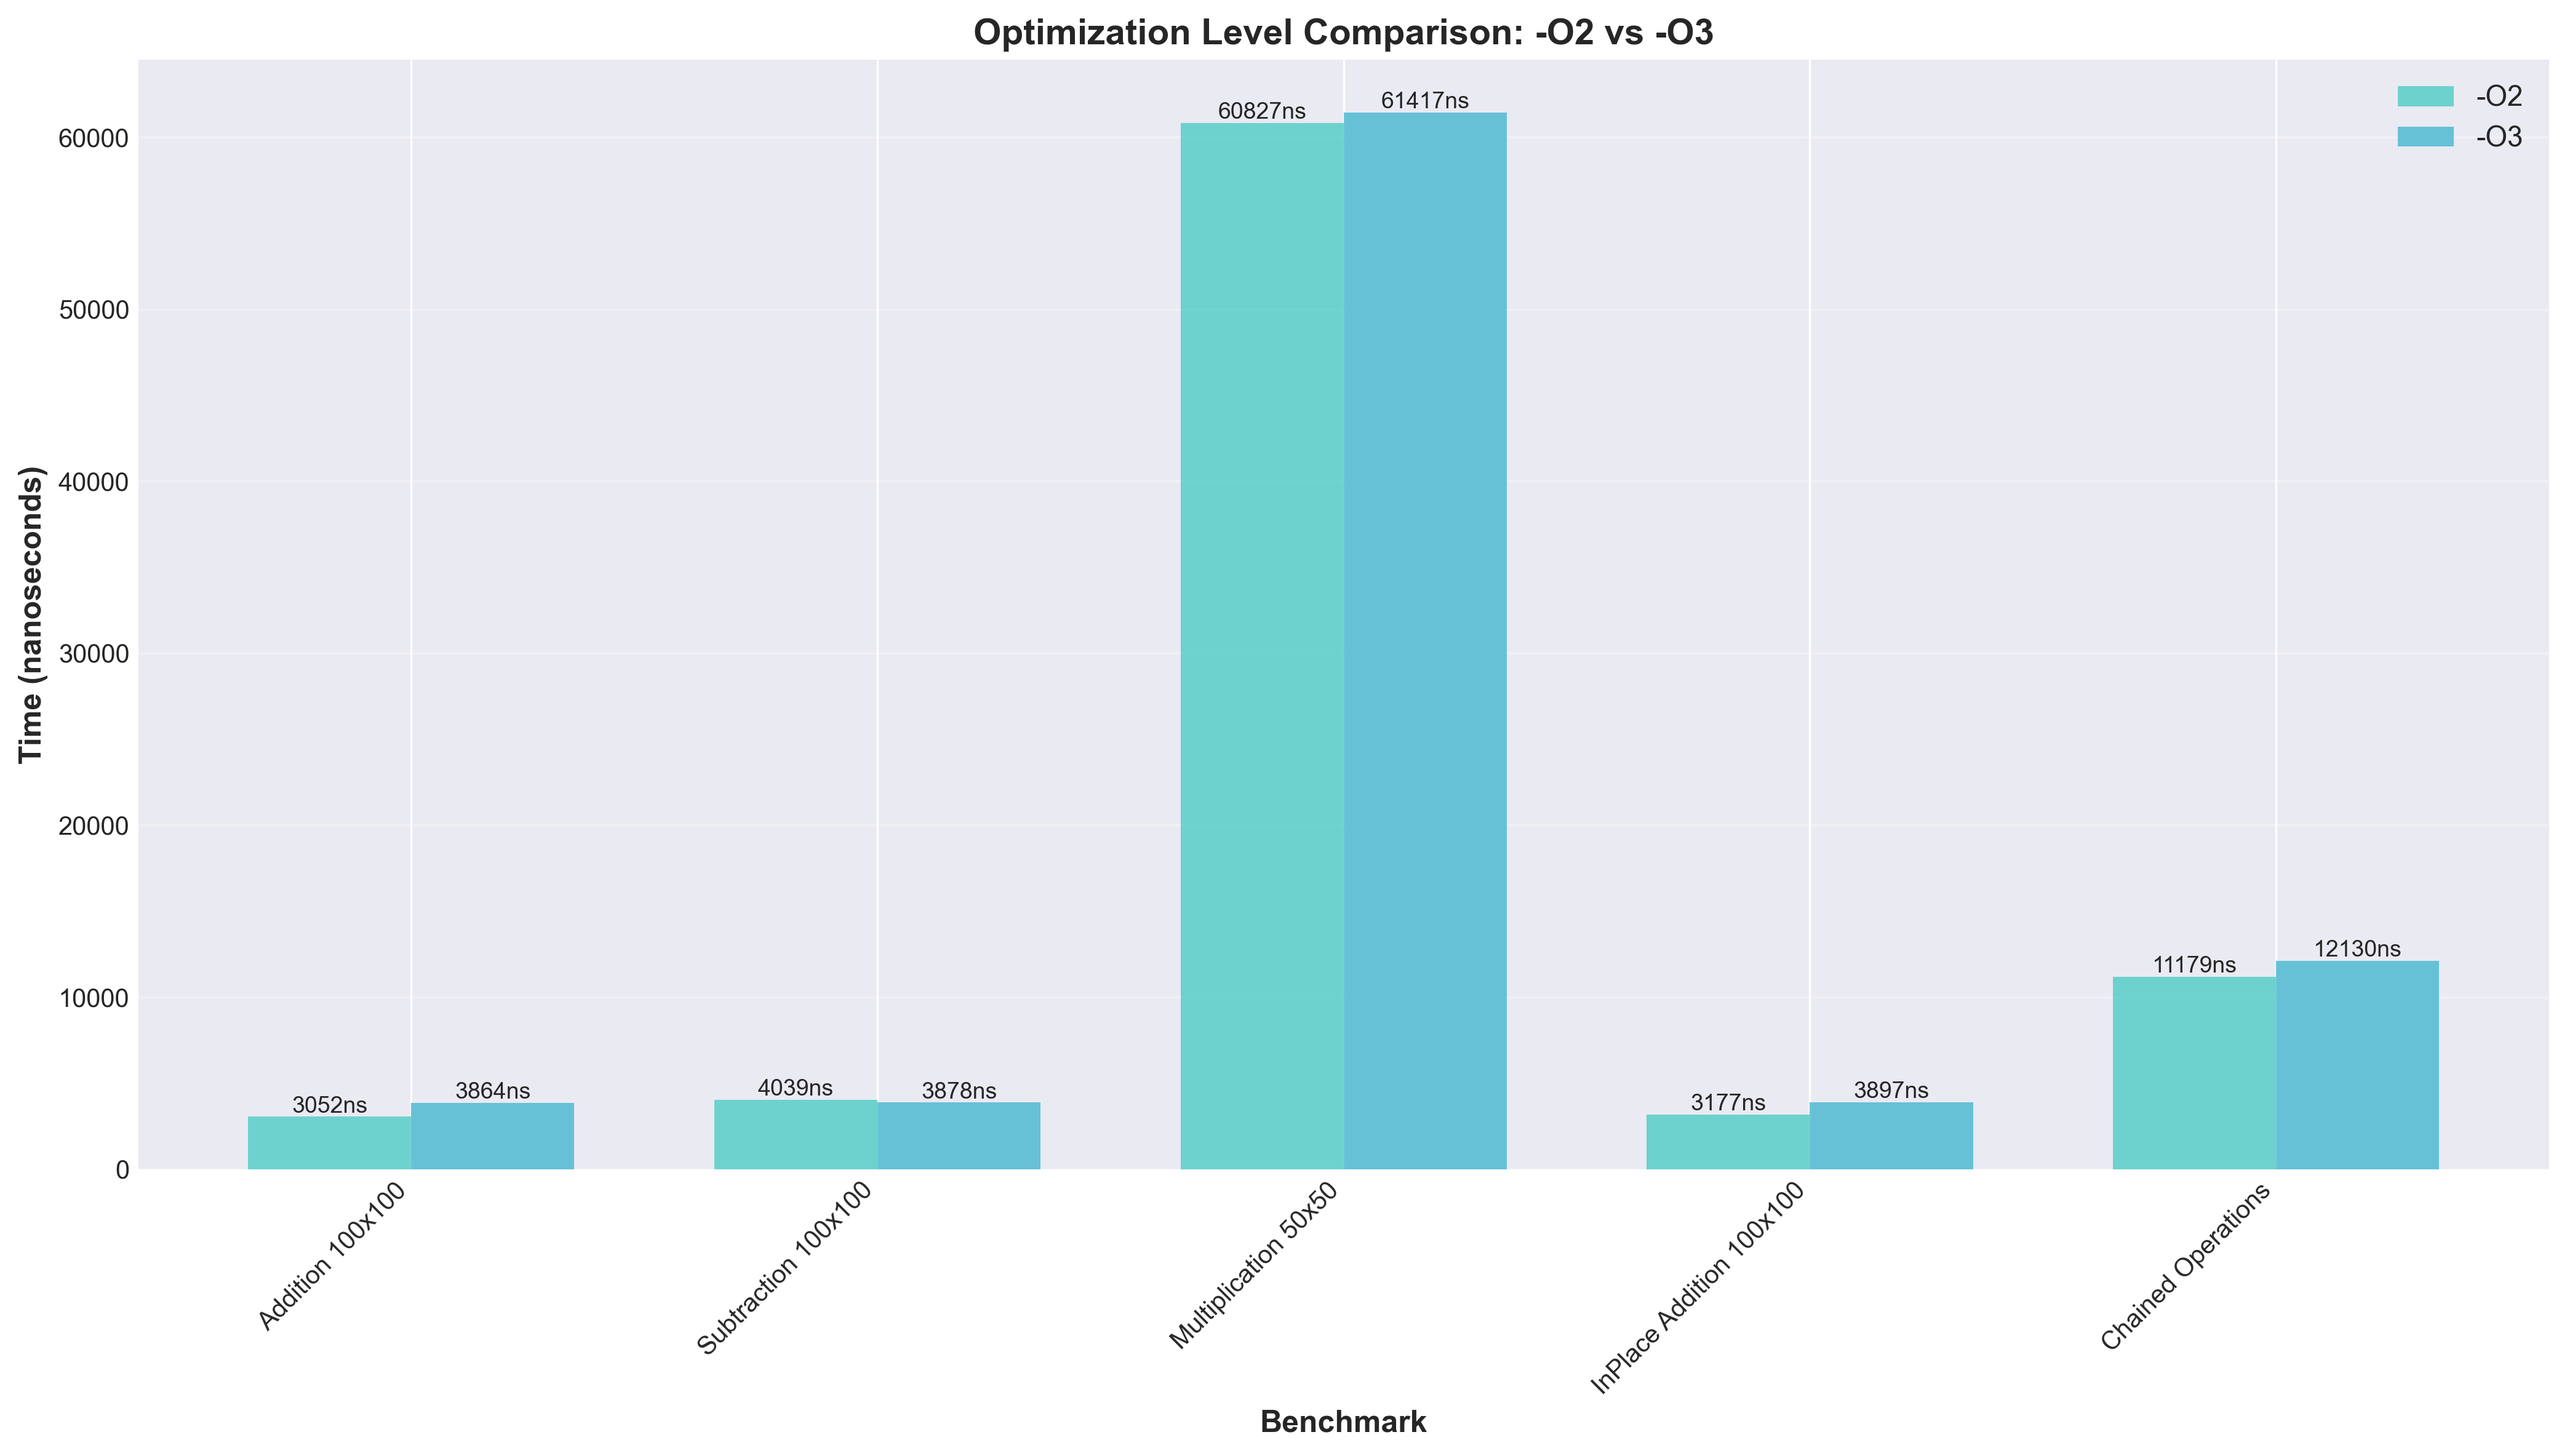
\includegraphics[width=0.9\textwidth]{charts/01_optimization_comparison.png}
  \caption{Laufzeitvergleich \texttt{-O2} gegenüber \texttt{-O3} für ausgewählte
  Operationen. Die höchste Optimierungsstufe bringt gegenüber \texttt{-O2}
  keinen durchgängigen Vorteil.}
  \label{fig:optlevels}
\end{figure}

Die Multiplikation dominiert das Laufzeitprofil deutlich: In einer gemischten
Arbeitslast aus Addition, Subtraktion, Multiplikation, in-place-Operation und
verketteten Ausdrücken entfällt der weitaus größte Anteil auf die
Multiplikation (Abbildung~\ref{fig:breakdown}). Dies entspricht der
Komplexität von $O(n^3)$ gegenüber $O(n^2)$ der übrigen Operationen.

\begin{figure}[H]
  \centering
  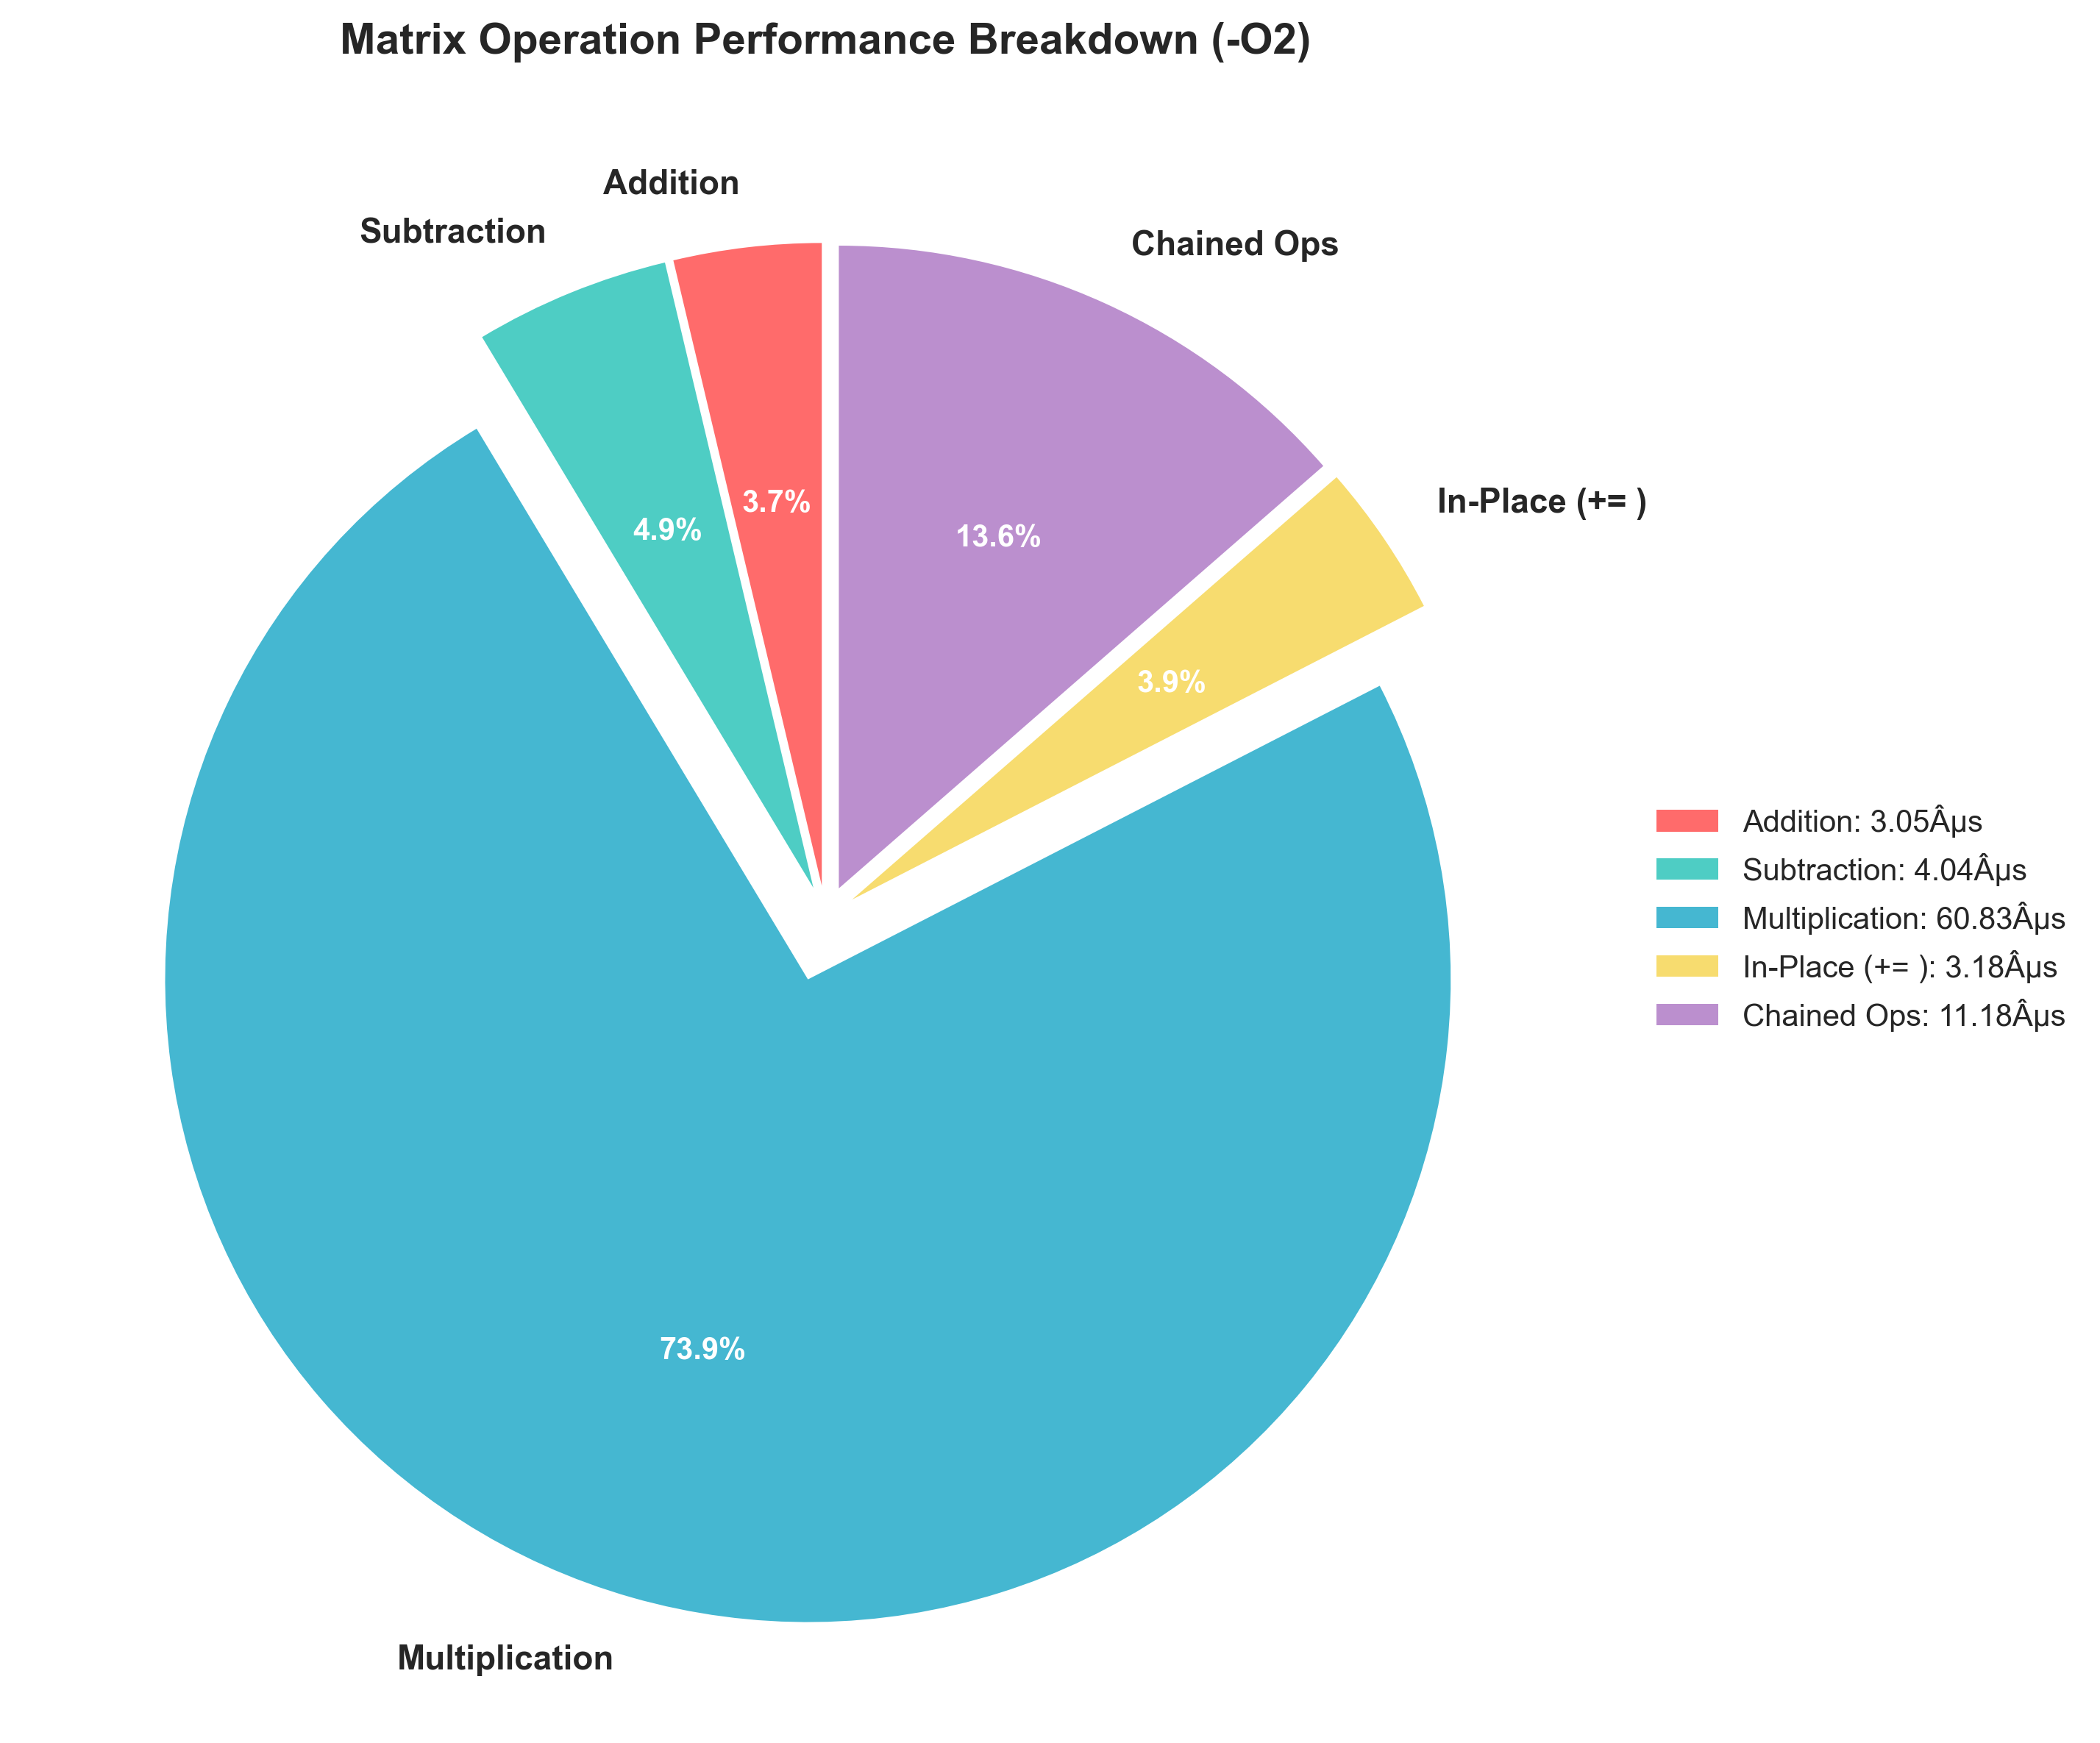
\includegraphics[width=0.75\textwidth]{charts/06_operation_breakdown.png}
  \caption{Anteil der Operationen an der Gesamtlaufzeit (\texttt{-O2}). Die
  Multiplikation überwiegt aufgrund ihrer kubischen Komplexität.}
  \label{fig:breakdown}
\end{figure}

Die Skalierung der Addition mit der Matrixgröße zeigt das erwartete
$O(n^2)$-Verhalten, allerdings überlagert von Cache-Effekten
(Tabelle~\ref{tab:skalierung}, Abbildung~\ref{fig:skalierung}). Beim Übergang von
$100\times100$ auf $500\times500$ wächst die Datenmenge um den Faktor~25, die
Laufzeit jedoch um etwa den Faktor~199. Eine $500\times500$-Matrix belegt rund
2\,MB und überschreitet damit den L2-Cache deutlich; die Operation wird
speicherbandbreitenbegrenzt. Der erweiterte Benchmark bestätigt diese Tendenz
bis $1000\times1000$ (rund 2{,}17\,ms bei \texttt{-O2}).

\begin{table}[htbp]
\centering
\caption{Laufzeit der Addition in Abhängigkeit von der Matrixgröße (\texttt{-O2}).}
\label{tab:skalierung}
\begin{tabular}{lrr}
\toprule
\textbf{Größe} & \textbf{Zeit} & \textbf{Faktor (ggü.\ $10\times10$)} \\
\midrule
$10\times10$   & 82\,ns    & 1 \\
$50\times50$   & 1\,135\,ns & 13{,}8 \\
$100\times100$ & 3\,052\,ns & 37{,}2 \\
$500\times500$ & 607\,987\,ns & 7\,414 \\
\bottomrule
\end{tabular}
\end{table}

\begin{figure}[H]
  \centering
  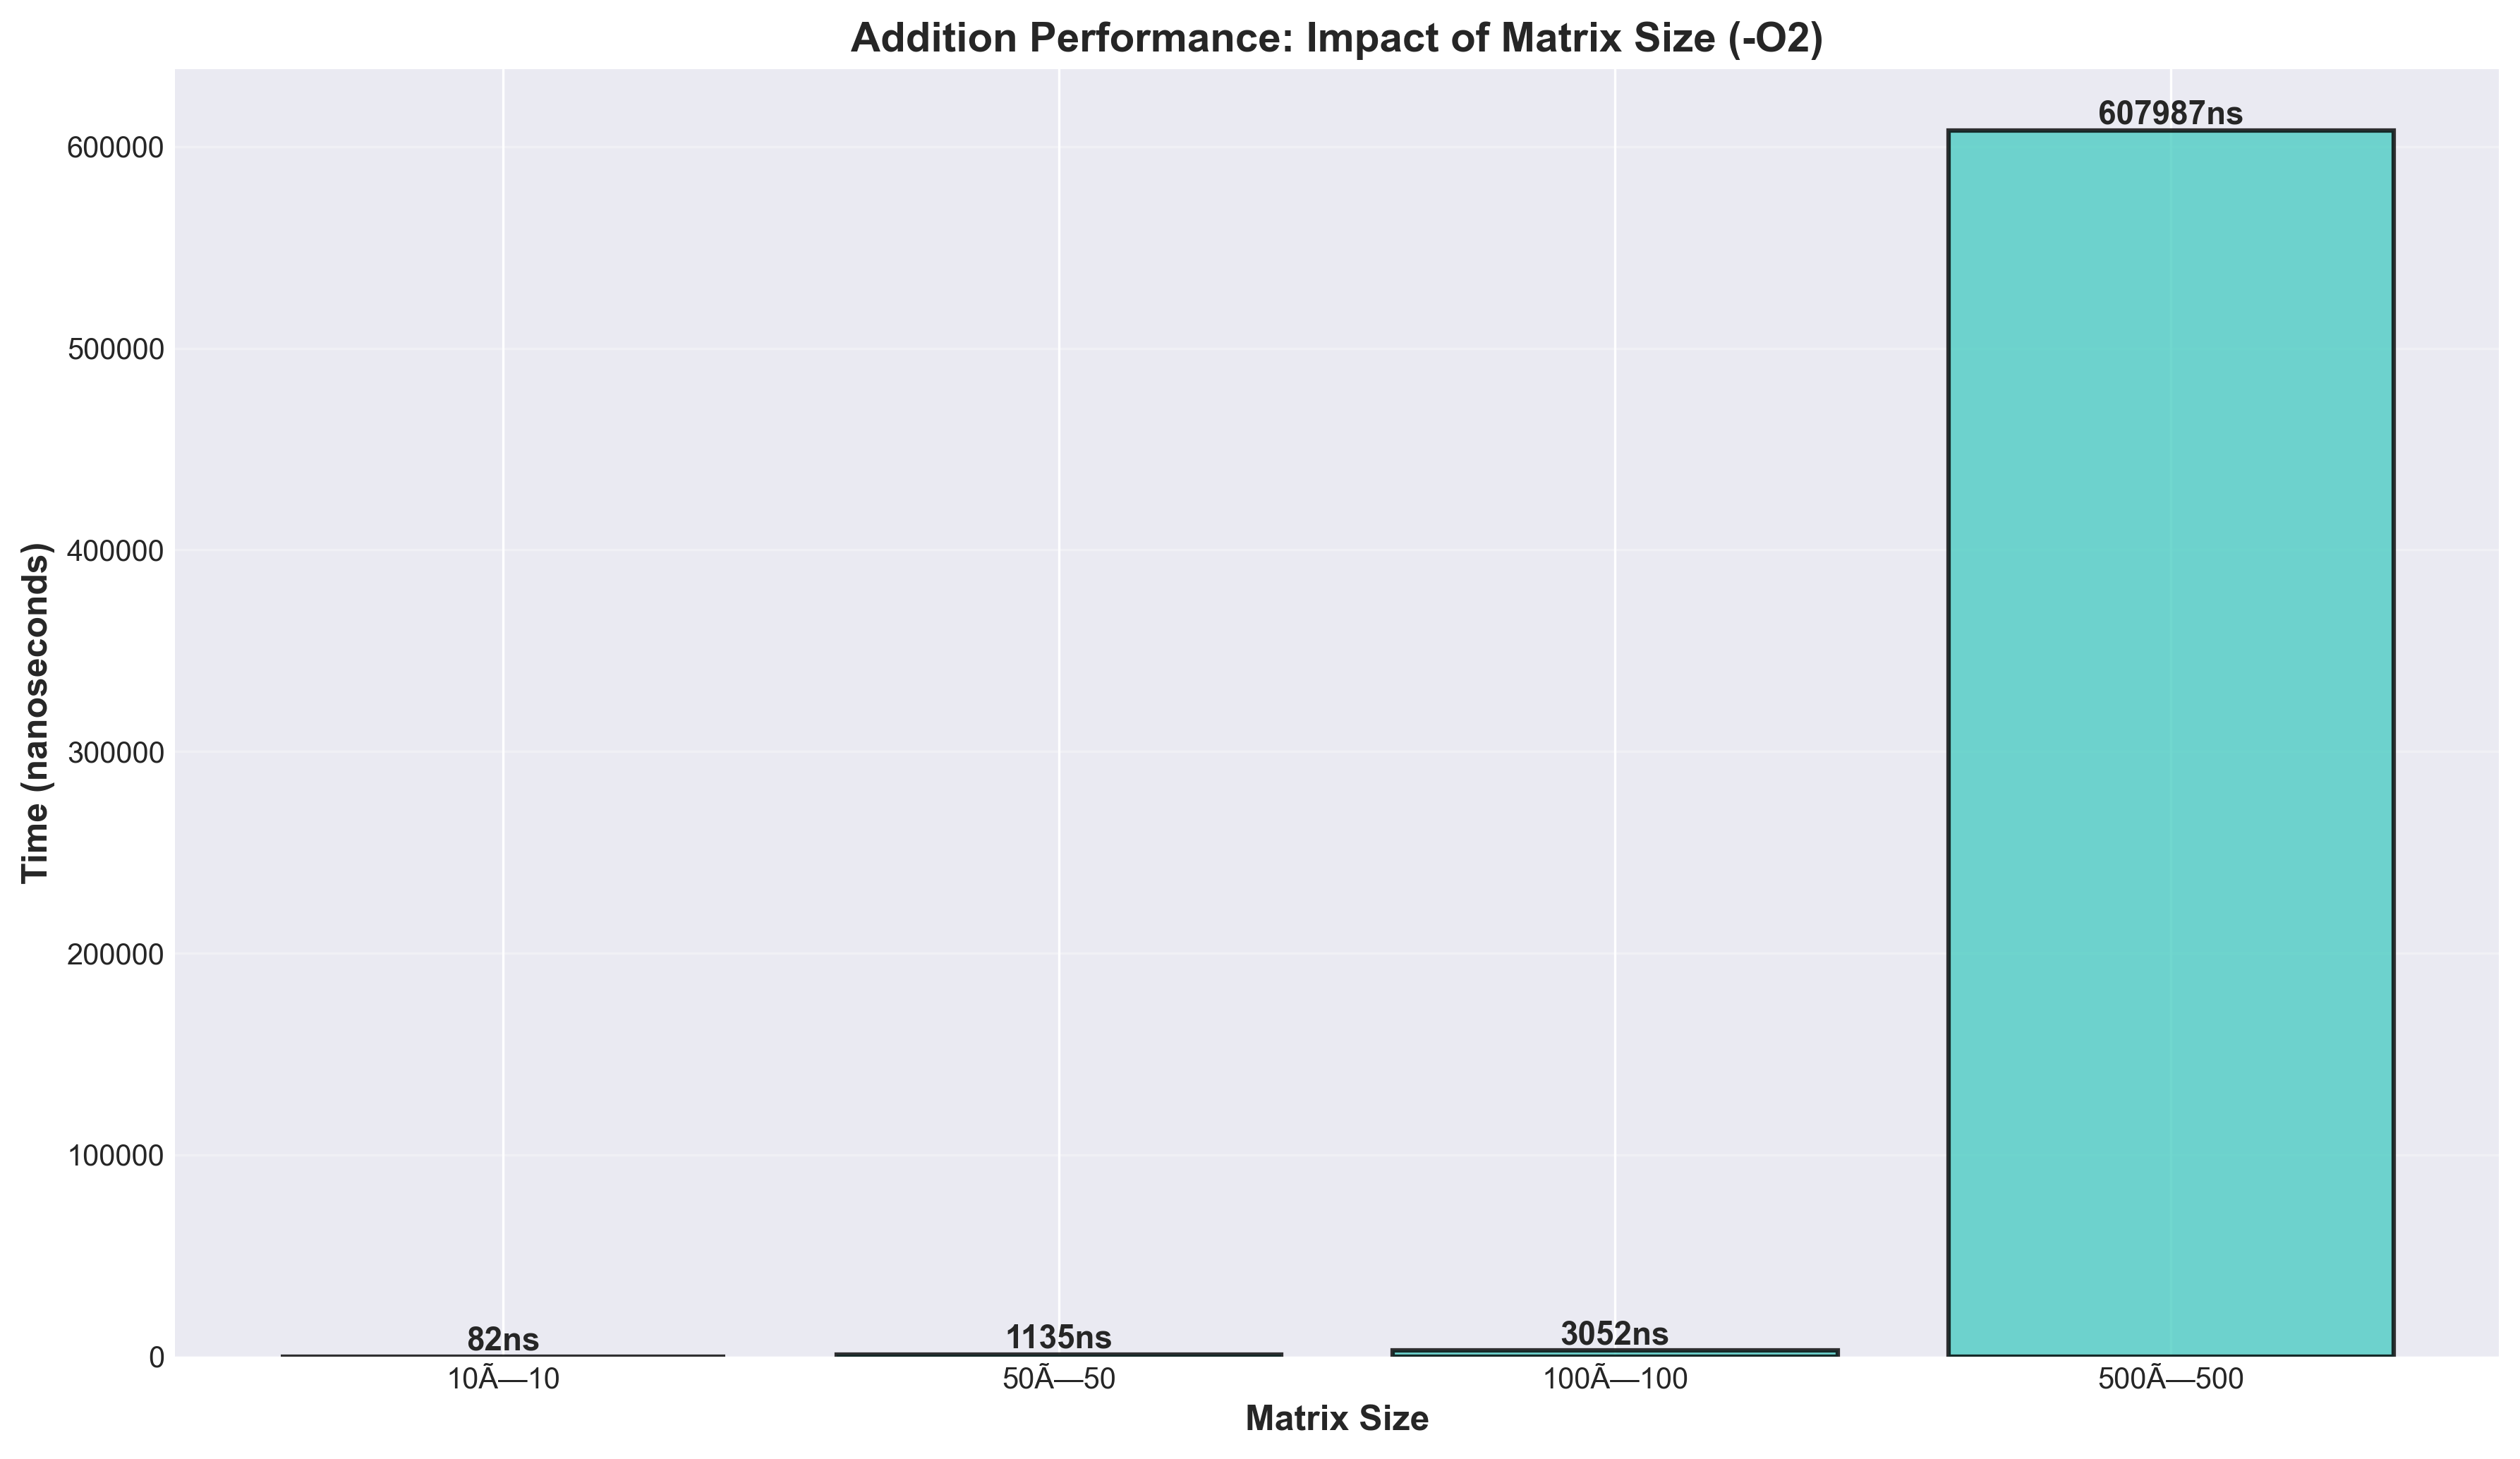
\includegraphics[width=0.85\textwidth]{./charts/02_matrix_size_impact.png}
  \caption{Laufzeit der Addition über die Matrixgröße (\texttt{-O2}). Der
  überproportionale Anstieg bei $500\times500$ ist auf Cache-Effekte
  zurückzuführen.}
  \label{fig:skalierung}
\end{figure}

Den belastbarsten Hinweis auf den Nutzen des in-place-Entwurfs liefert der
direkte Vergleich von freier Funktion (\texttt{A + B}) und in-place-Operator
(\texttt{A += B}). Bei $100\times100$ ist die in-place-Variante etwa 25\,\%
schneller (3{,}46\,$\mu$s gegenüber 4{,}61\,$\mu$s), bei $500\times500$ rund das
2{,}6-Fache (235\,$\mu$s gegenüber 609\,$\mu$s). Der Unterschied entspricht
gerade jener einen Kopie des linken Operanden, die \texttt{operator+} intern
anlegt (Listing~\ref{lst:v3}) und die \texttt{operator+=} einspart. Bei sehr
kleinen Matrizen ($10\times10$) kehrt sich das Bild messtechnisch um; dieser
Effekt ist jedoch auf den in Abschnitt~\ref{sec:methodik} beschriebenen
Pausierungs-Aufwand zurückzuführen und nicht auf die Operation selbst.

\subsection{Ergebnisse: Temporäre Objekte}
\label{sec:tempobjekte}

Tabelle~\ref{tab:temporaries} weist die je Operation erzeugten Kopien und Moves
aus. Bemerkenswert ist, dass über alle Operationen hinweg kein einziger Move
gezählt wird. Dies ist kein Widerspruch zur vorhandenen Move-Semantik, sondern
eine unmittelbare Folge der Kopierauslassung: Die freie Funktion
\texttt{operator+} gibt eine benannte lokale Variable zurück (NRVO), und am
Aufrufort initialisiert ein prvalue das Ergebnisobjekt (garantierte Elision).
Beide Mechanismen entfernen den Rückgabe-Move vollständig. Die gezählten Kopien
stammen daher nicht aus der Rückgabe, sondern aus der einen Kopie des linken
Operanden innerhalb von \texttt{operator+} bzw.\ aus der bewussten Kopie zur
Vorbereitung der in-place-Messung.

\begin{table}[htbp]
\centering
\caption{Kopien und Moves je Operation (instrumentierte Zählung).}
\label{tab:temporaries}
\begin{tabular}{lrr}
\toprule
\textbf{Operation} & \textbf{Kopien / Op.} & \textbf{Moves / Op.} \\
\midrule
Addition ($A+B$)            & 1 & 0 \\
Subtraktion ($A-B$)         & 1 & 0 \\
Multiplikation ($A \cdot B$)& 0 & 0 \\
In-place ($\mathit{temp}=A;\ \mathit{temp}{+}{=}B$) & 1 & 0 \\
Verkettet ($A+B+C$)         & 2 & 0 \\
Gemischt                    & 2 & 0 \\
\bottomrule
\end{tabular}
\end{table}

Damit bestätigt sich die theoretische Vorhersage aus Abschnitt~2.6: Verkettete
Ausdrücke erzeugen proportional mehr Kopien (zwei statt einer), während die
Multiplikation -- die ihr Ergebnis intern aufbaut, ohne den linken Operanden zu
kopieren -- ganz ohne Kopie auskommt. Abbildung~\ref{fig:temporaries} stellt die
absoluten Zählwerte dar; da Google Benchmark je Operation unterschiedlich viele
Iterationen ausführt, sind für den Vergleich die Werte \emph{pro Operation} aus
Tabelle~\ref{tab:temporaries} maßgeblich.

\begin{figure}[H]
  \centering
  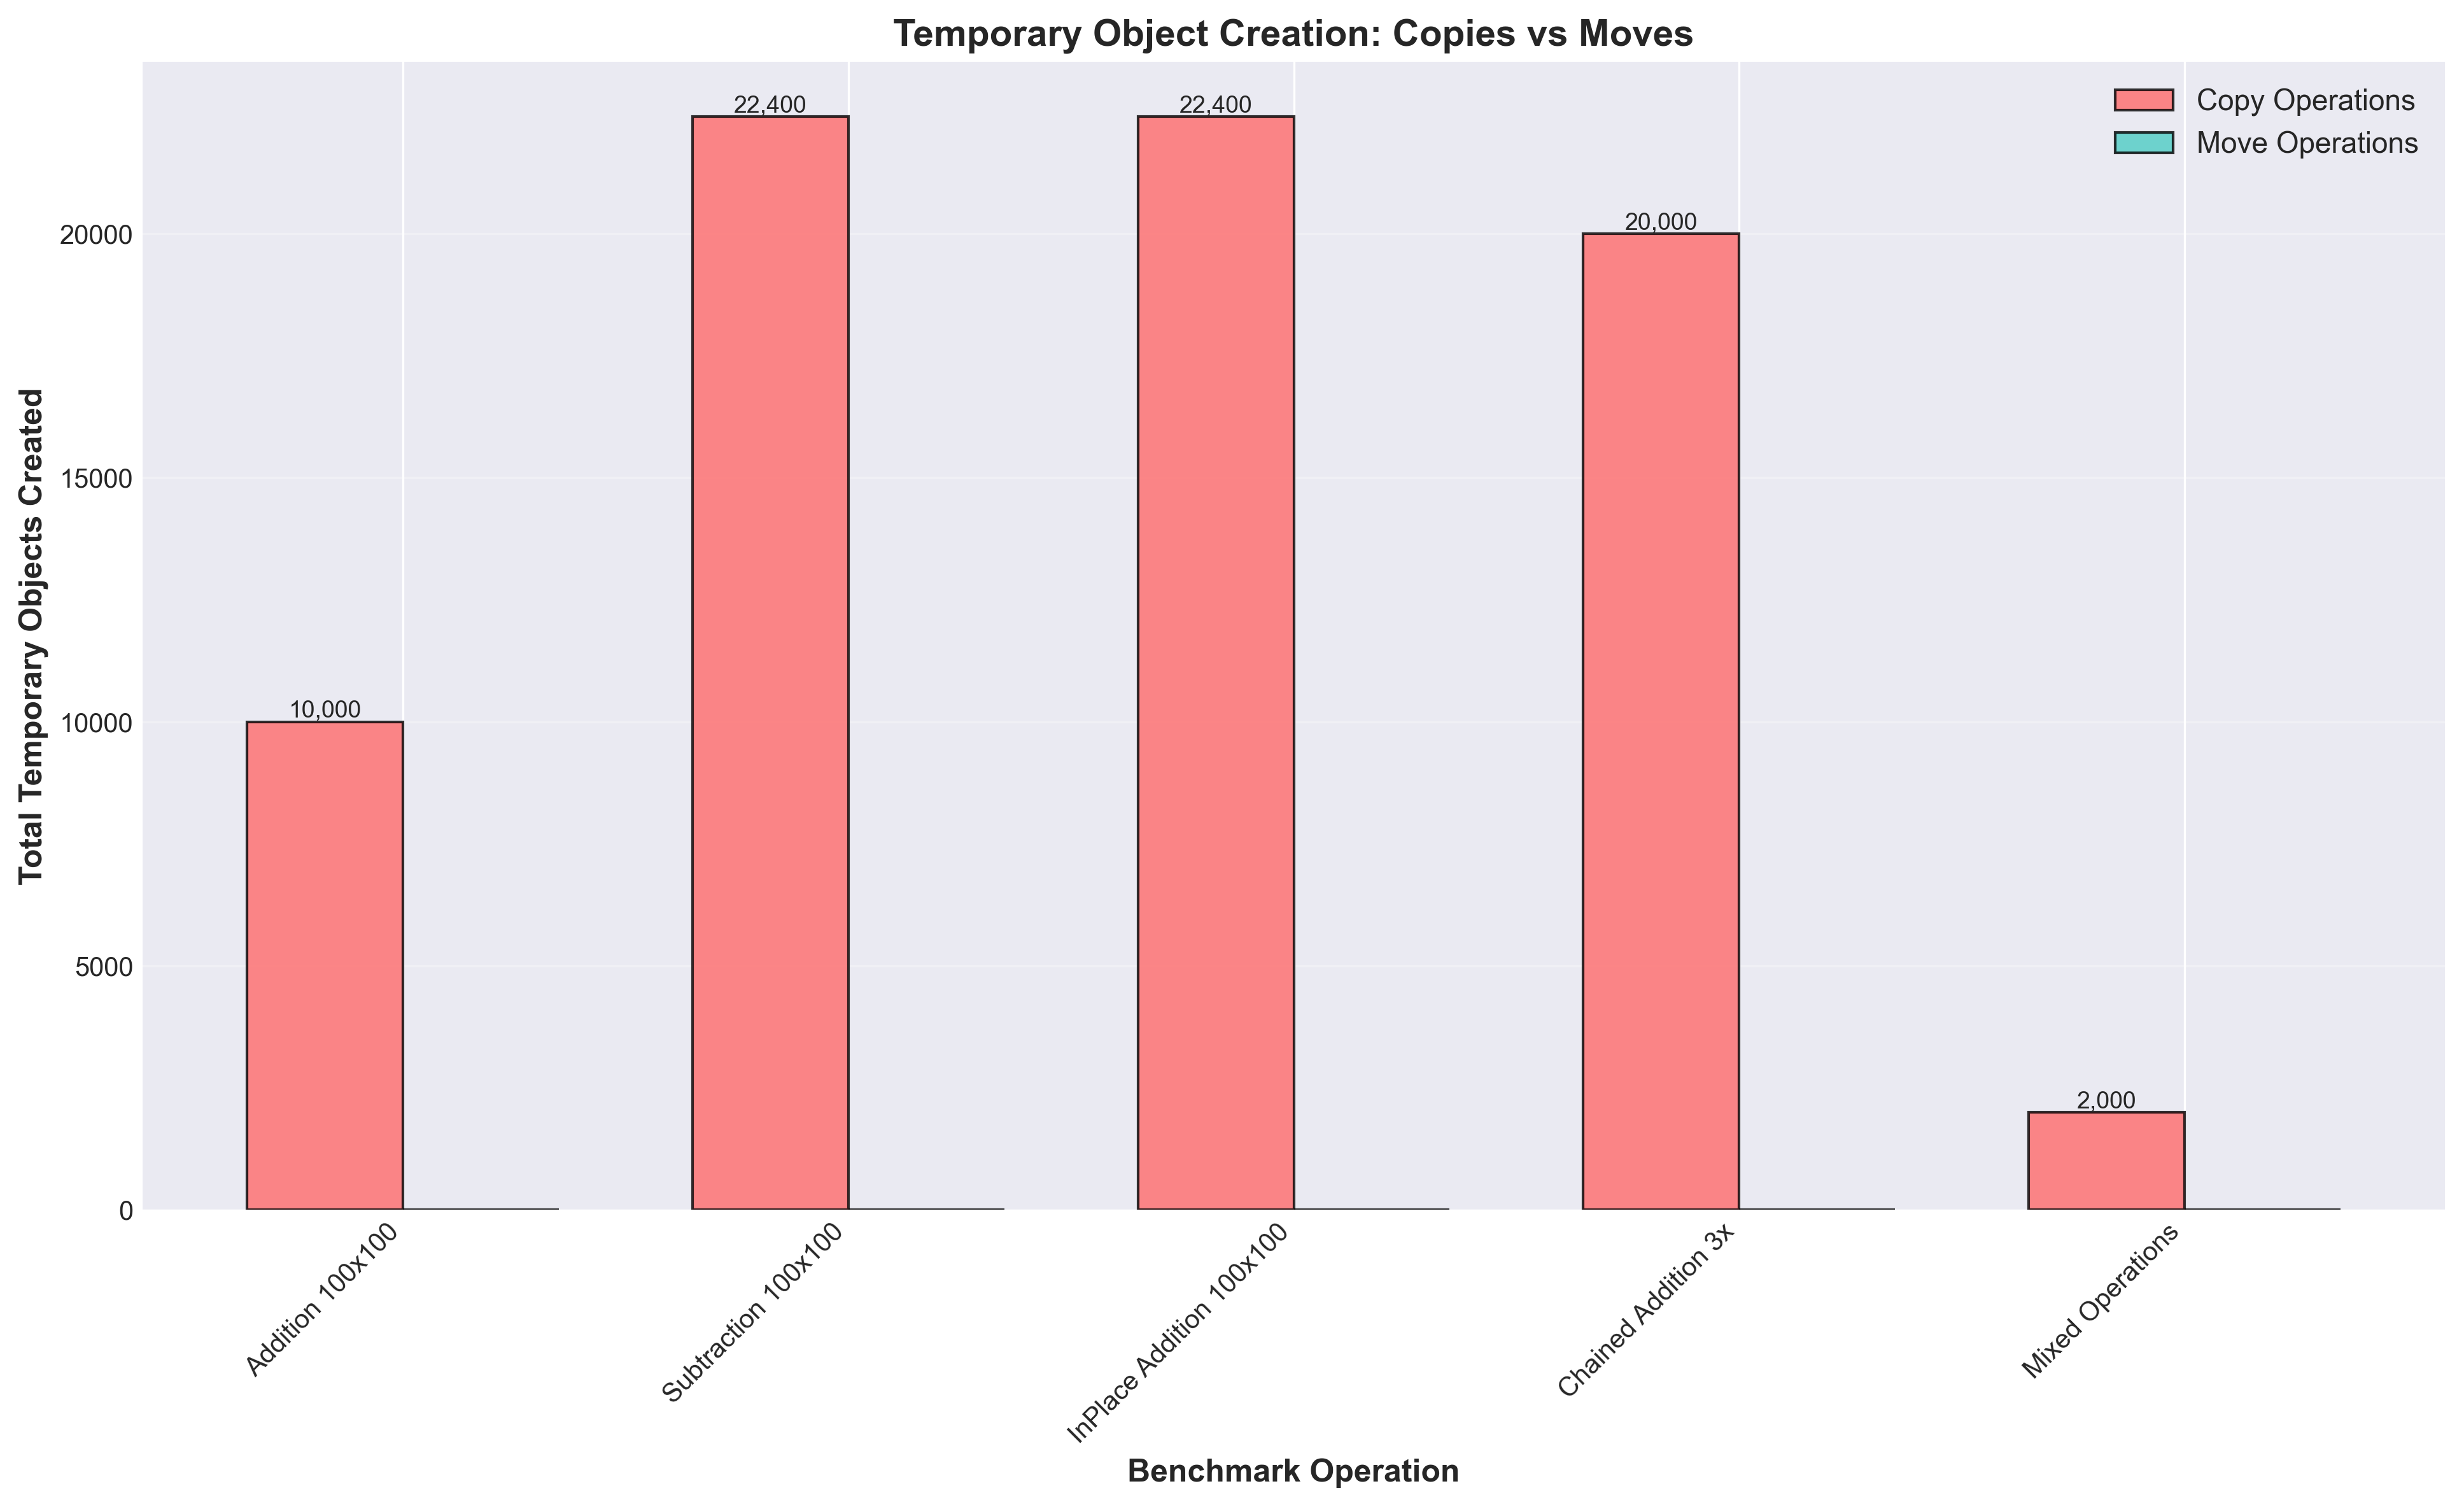
\includegraphics[width=0.85\textwidth]{./charts/04_temporary_objects.png}
  \caption{Erzeugte temporäre Objekte (Kopien gegenüber Moves). Die
  Move-Operationen entfallen aufgrund der Kopierauslassung vollständig.}
  \label{fig:temporaries}
\end{figure}

\subsection{Ergebnisse: Speicherverbrauch}
\label{sec:speicher}

Das Speicherverhalten wird anhand der Kopier- und Move-Zähler in fünf
Szenarien untersucht (Tabelle~\ref{tab:heap}). Da die vereinheitlichte Klasse
Move-Semantik besitzt, gibt die Spalte ``gemessen'' die tatsächlich gezählten
Operationen wieder; die Spalte ``V1-Schätzung'' gibt analytisch an, wie viele
tiefe Kopien dieselben Szenarien ohne Move-Semantik verursachen würden (jede
Move-Operation wird dann zu einer Kopie).

\begin{table}[htbp]
\centering
\caption{Kopier- und Move-Operationen je Szenario (instrumentierte Zählung;
V1-Spalte als analytische Schätzung).}
\label{tab:heap}
\begin{tabular}{lrrr}
\toprule
\textbf{Szenario} & \textbf{Kopien} & \textbf{Moves} & \textbf{V1-Schätzung (Kopien)} \\
\midrule
Einfache Addition ($m_3 = m_1+m_2$)     & 1 & 1 & 2 \\
Verkettete Addition ($m_4 = m_1+m_2+m_3$) & 2 & 1 & 3 \\
Akkumulation (\texttt{+=}, 100$\times$)  & 0 & 0 & 100 \\
Vektor (100 Matrizen)                    & 100 & 127 & $>100$ \\
Temporäre Ausdrücke (1000$\times$)       & 2\,000 & 1\,000 & 3\,000 \\
\bottomrule
\end{tabular}
\end{table}

Die Akkumulationsschleife mit \texttt{operator+=} kommt ohne jede Kopie und
ohne jeden Move aus -- die Datenmengen werden ausschließlich in-place addiert.
Ohne zusammengesetzten Operator (\texttt{result = result + temp;}) wären je
Iteration eine Kopie und eine Zuweisung nötig. Beim Einfügen in einen
\texttt{std::vector} treten neben den 100 Kopien der Elemente zusätzliche
Move-Operationen bei den Reallokationen des Vektors auf; diese sind nur möglich,
weil der Move-Konstruktor \texttt{noexcept} ist (Abschnitt~2.4).
Abbildung~\ref{fig:heap} stellt die gemessenen Operationen der vereinheitlichten
Klasse der analytischen V1-Schätzung gegenüber.

\begin{figure}[H]
  \centering
  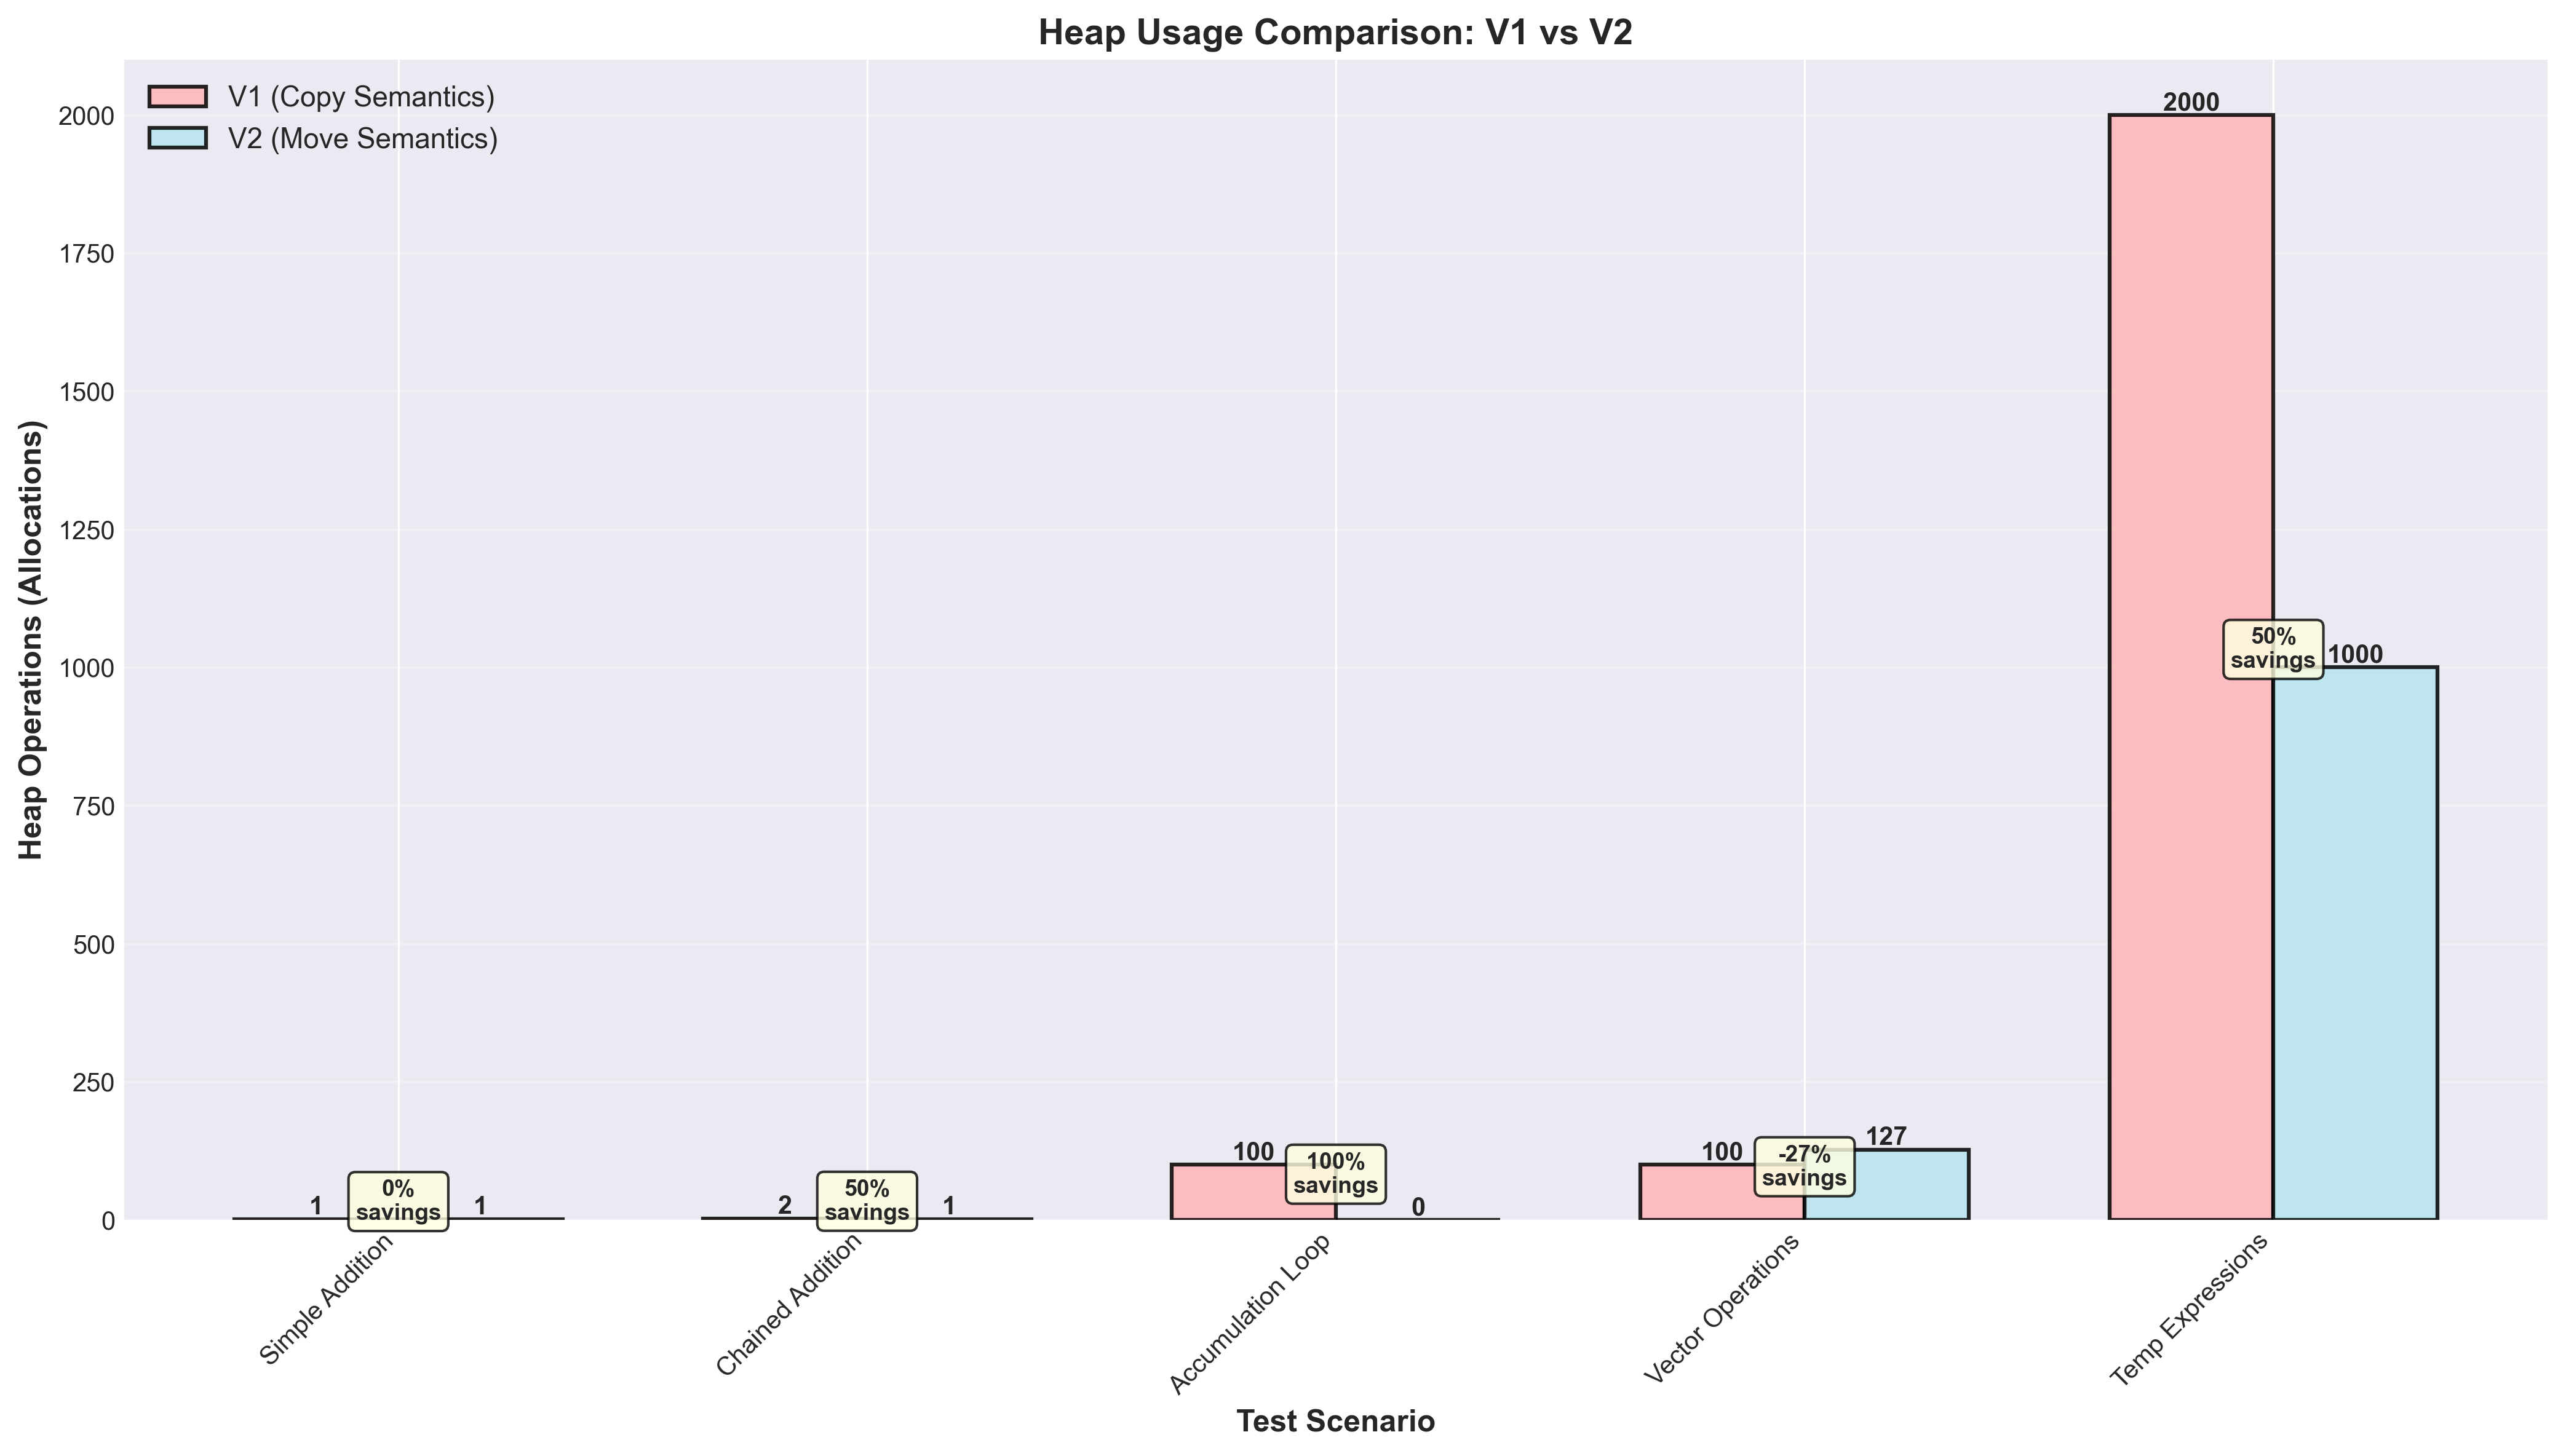
\includegraphics[width=0.85\textwidth]{./charts/05_heap_usage_comparison.png}
  \caption{Kopier- und Move-Operationen je Szenario (V1 als analytische
  Schätzung gegenüber der move-fähigen Implementierung V2).}
  \label{fig:heap}
\end{figure}

\subsection{Interpretation der Ergebnisse}
\label{sec:interpretation}

Die Ergebnisse lassen sich zu vier belastbaren Aussagen verdichten.

\emph{Erstens} dominiert die algorithmische Komplexität die Laufzeit weit stärker
als der Entwurf der Operatoren. Die Multiplikation ($O(n^3)$) übersteigt
Addition und Subtraktion ($O(n^2)$) um mehr als eine Größenordnung und bestimmt
das Laufzeitprofil gemischter Arbeitslasten (Abbildung~\ref{fig:breakdown}).

\emph{Zweitens} liegt der mit Abstand größte Optimierungsgewinn im Übergang von
\texttt{-O0} zu \texttt{-O2}, während \texttt{-O3} keinen verlässlichen
Zusatznutzen bringt. Die Optimierungsstufe wirkt auf die Berechnungsschleifen,
nicht auf die Objektverwaltung; beide Achsen sind weitgehend unabhängig.

\emph{Drittens} zeigt sich der praktische Nutzen des in-place-Entwurfs am
deutlichsten dort, wo die Messung nicht durch den Pausierungs-Aufwand verfälscht
wird: Bei $500\times500$ ist \texttt{+=} rund 2{,}6-mal schneller als das freie
\texttt{+}, da letzteres eine vollständige Kopie des linken Operanden anlegt.
Dies ist der unmittelbar messbare Vorteil von Version~3 gegenüber Version~2.

\emph{Viertens} bestätigt die Zählung der temporären Objekte die theoretische
Erwartung: Unter C++17 entfernt die Kopierauslassung sämtliche Rückgabe-Moves,
weshalb sich naive und move-fähige Implementierungen bei der direkten
Initialisierung (\texttt{Matrix D = A + B;}) kaum unterscheiden. Der Nutzen der
Move-Semantik verlagert sich damit auf die Zuweisung aus temporären Objekten,
auf verkettete Ausdrücke und insbesondere auf Container-Reallokationen, wie
Tabelle~\ref{tab:heap} zeigt.

Einschränkend ist festzuhalten, dass die direkten Mikrobenchmarks von
Kopier- gegen Move-Konstruktor (gemessen 1\,523\,ns gegenüber 1\,175\,ns) und
von Kopier- gegen Move-Zuweisung (1\,382\,ns gegenüber 1\,552\,ns,
Abbildung~\ref{fig:copymove}) den theoretisch erwarteten großen Vorsprung der
Move-Operationen \emph{nicht} widerspiegeln. Ursache ist der in
Abschnitt~\ref{sec:methodik} beschriebene Pausierungs-Aufwand, der die wenige
Nanosekunden dauernde Zeigerübernahme überdeckt. Der eigentliche Beleg für den
Nutzen der Move-Semantik liegt daher nicht in diesen Einzelmessungen, sondern in
der Kombination aus den Operationszählungen (Tabelle~\ref{tab:temporaries},
\ref{tab:heap}) und dem skalierungsabhängigen Vorteil des in-place-Entwurfs.

\begin{figure}[H]
  \centering
  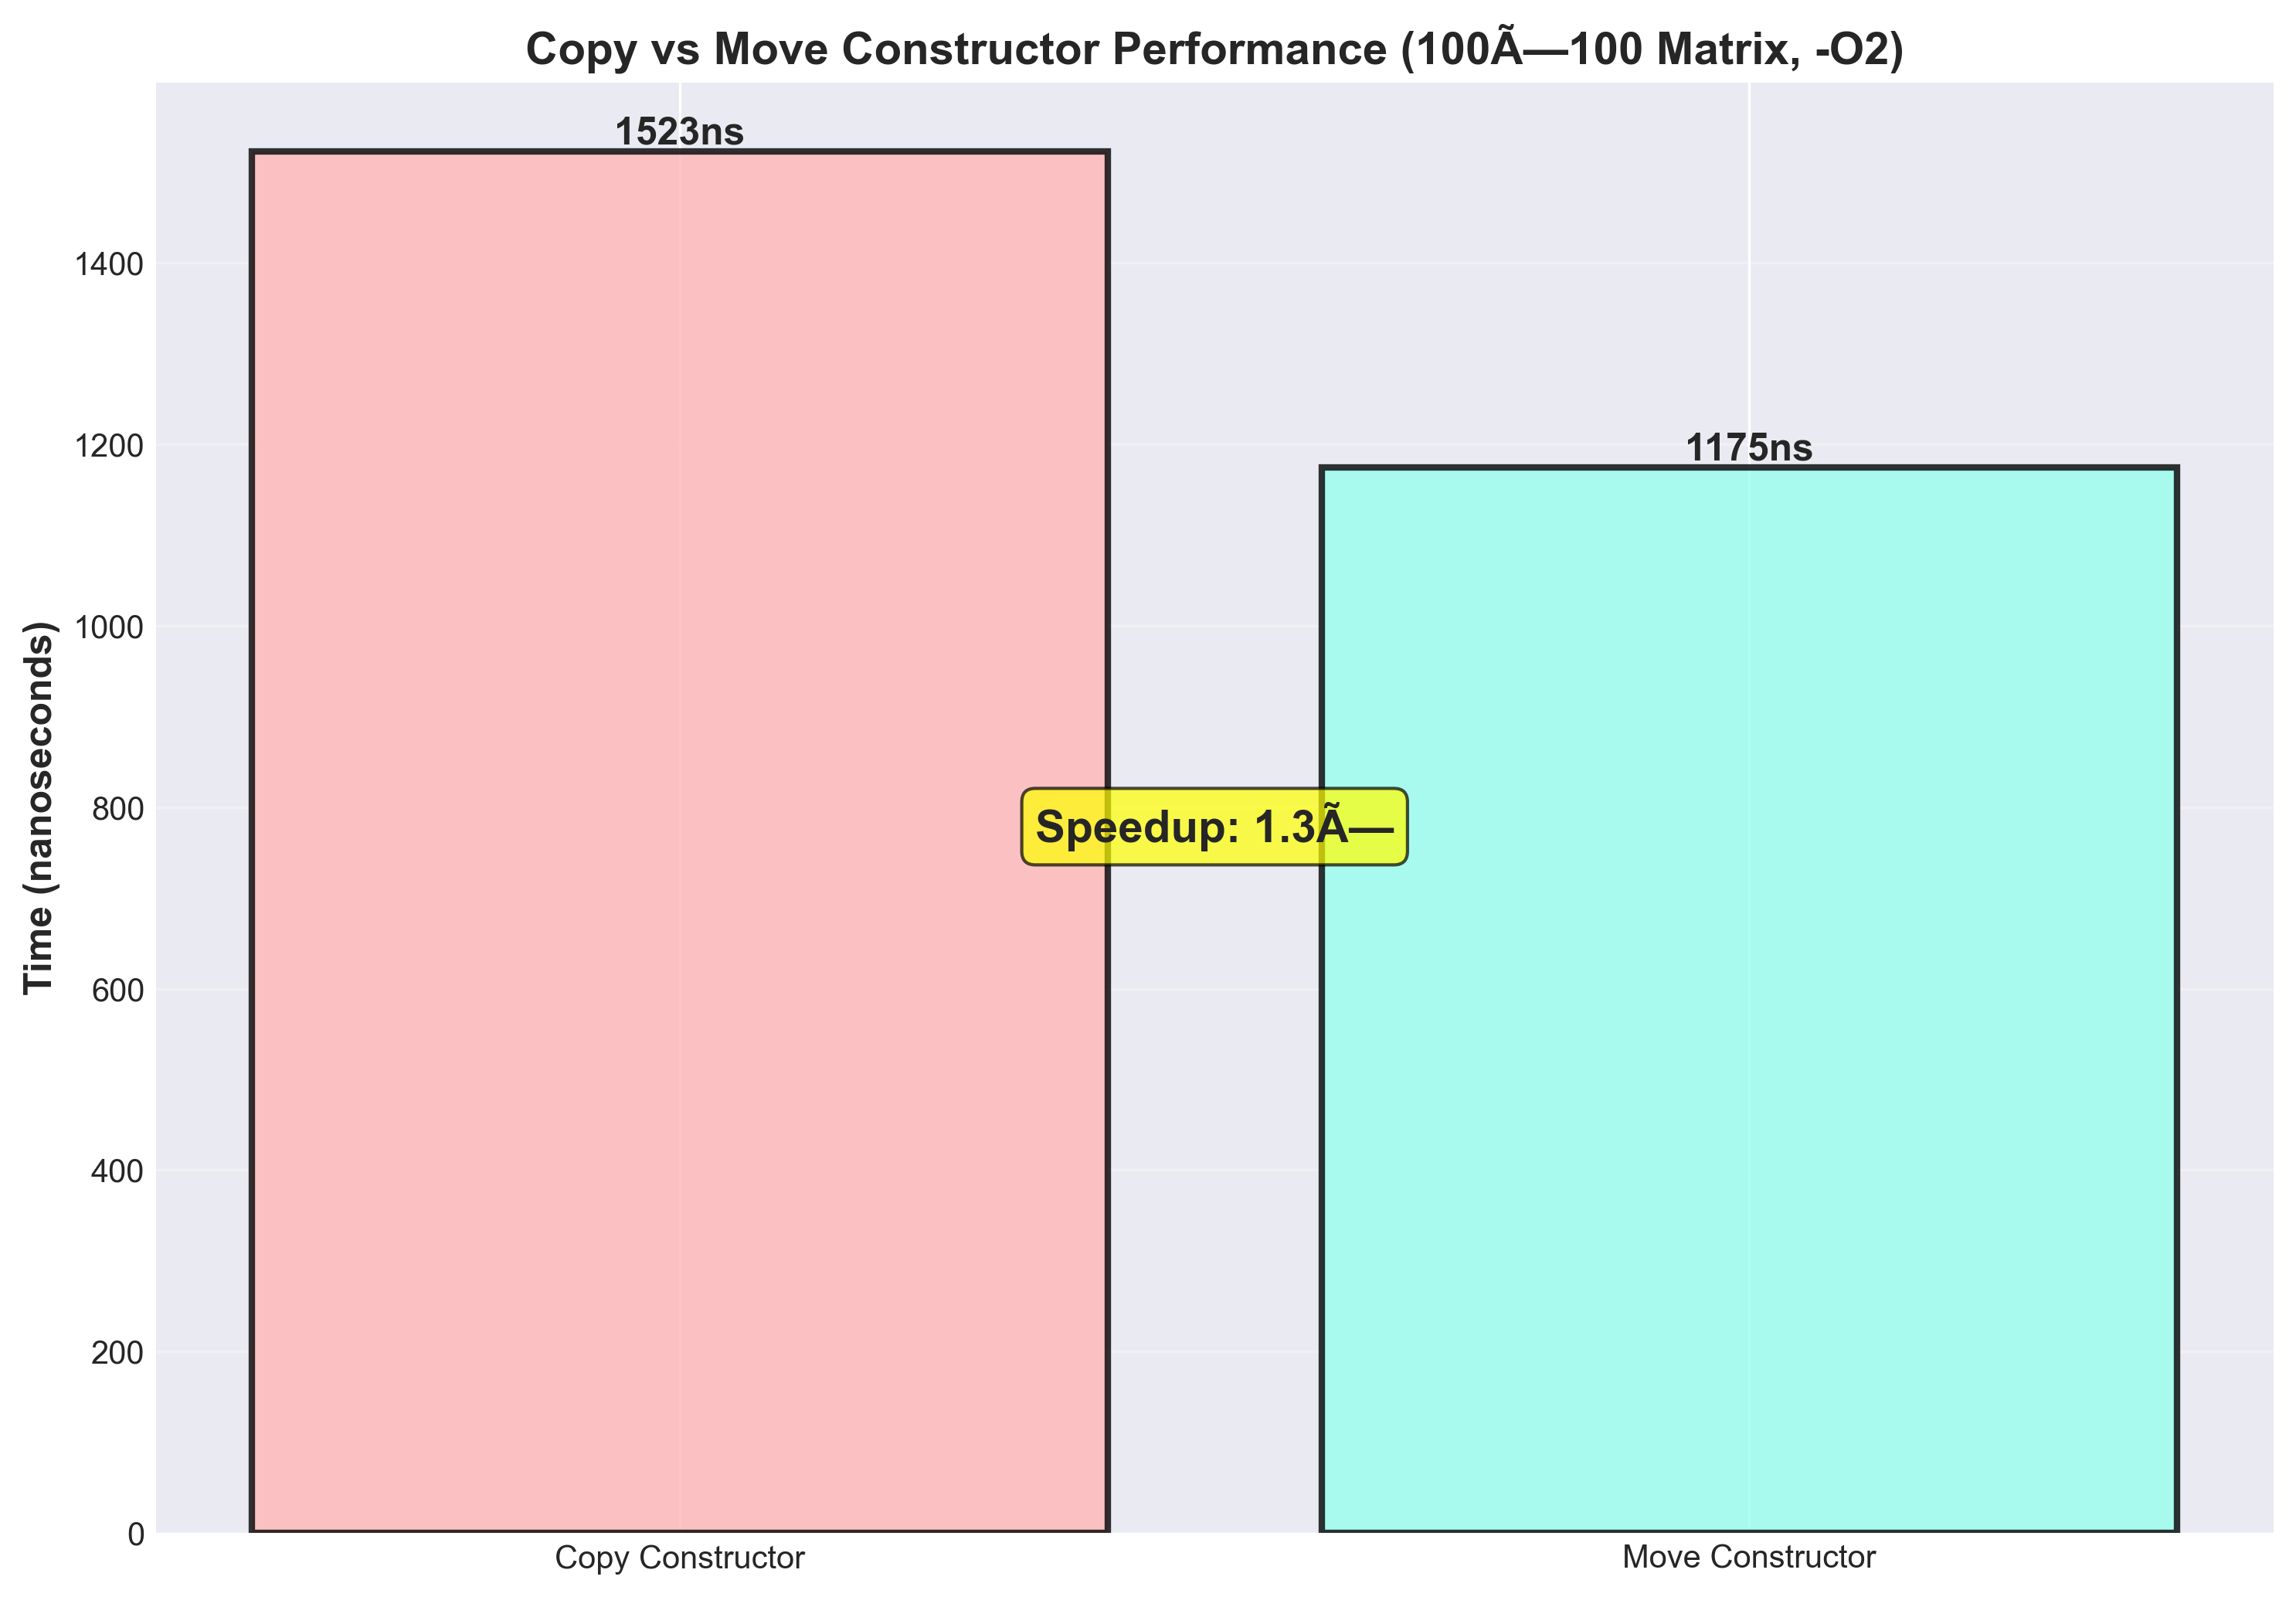
\includegraphics[width=0.7\textwidth]{./charts/03_copy_vs_move.png}
  \caption{Kopier- gegenüber Move-Konstruktor ($100\times100$, \texttt{-O2}).
  Der geringe gemessene Abstand ist durch den Pausierungs-Aufwand des
  Messrahmens bedingt und unterschätzt den tatsächlichen Vorteil der
  Move-Operation.}
  \label{fig:copymove}
\end{figure}

% ------------------------------------------------------------
% ============================================================
%  ERSATZ FUER ABSCHNITT 5 (Fazit)
%  Einfuegen anstelle des bisherigen Platzhalter-Abschnitts.
% ============================================================
 
% ------------------------------------------------------------
\section{Fazit}
\label{sec:fazit}
 
\subsection{Zusammenfassung}
\label{sec:zusammenfassung}
 
Die vorliegende Arbeit hat das Überladen von Operatoren in C++ zunächst
theoretisch dargestellt und seine Effizienzaspekte anschließend am Beispiel
einer Matrix-Klasse empirisch untersucht. Ausgangspunkt war die Beobachtung,
dass die syntaktische Eleganz überladener Operatoren erhebliche, im Quelltext
nicht unmittelbar sichtbare Kosten verbergen kann -- die Erzeugung temporärer
Objekte, tiefe Kopien und wiederholte Heap-Allokationen. Die Untersuchung ging
der Frage nach, unter welchen Bedingungen unterschiedliche
Implementierungsvarianten (naive Kopiersemantik, Move-Semantik und
zusammengesetzte Operatoren) diese Kosten tatsächlich beeinflussen.
 
Die Ergebnisse lassen sich in vier Aussagen zusammenfassen. \emph{Erstens}
dominiert die algorithmische Komplexität die Laufzeit weit stärker als der
Entwurf der Operatoren: Die Multiplikation mit $O(n^3)$ übersteigt die
elementweisen Operationen mit $O(n^2)$ um mehr als eine Größenordnung.
\emph{Zweitens} liegt der größte Optimierungsgewinn im Übergang von
\texttt{-O0} zu \texttt{-O2} (Faktor~6 bis~13), während \texttt{-O3} keinen
verlässlichen Zusatznutzen bringt; die Optimierung wirkt auf die
Berechnungsschleifen, nicht auf die Objektverwaltung. \emph{Drittens} entfernt
die seit C++17 verpflichtende Kopierauslassung sämtliche Rückgabe-Moves,
weshalb sich naive und move-fähige Implementierungen bei der direkten
Initialisierung (\texttt{Matrix D = A + B;}) praktisch nicht unterscheiden --
in den Messungen wurde kein einziger Move gezählt. Der Nutzen der Move-Semantik
verlagert sich damit auf die Zuweisung aus temporären Objekten, auf verkettete
Ausdrücke und vor allem auf Container-Reallokationen. \emph{Viertens} zeigt sich
der praktische Vorteil des in-place-Entwurfs am deutlichsten beim Vergleich von
freier Funktion und zusammengesetztem Operator: Bei einer
$500\times500$-Matrix ist \texttt{+=} rund 2{,}6-mal schneller als das freie
\texttt{+}, da Letzteres eine vollständige Kopie des linken Operanden anlegt,
die \texttt{+=} einspart.
 
Damit bestätigt sich die Ausgangsthese in präzisierter Form: Lesbarer und
performanter Code sind nicht zwangsläufig identisch, lassen sich aber durch
geeignete Entwurfstechniken miteinander vereinbaren. Move-Semantik,
zusammengesetzte Operatoren und das Vertrauen auf die compilerseitige
Kopierauslassung erlauben es, die ausdrucksstarke Operatorsyntax beizubehalten,
ohne ihre verborgenen Kosten in Kauf nehmen zu müssen. Einschränkend ist
festzuhalten, dass einige Mikrobenchmarks -- insbesondere der direkte Vergleich
von Kopier- und Move-Operationen -- durch den Aufwand des Messrahmens überlagert
werden und den theoretischen Vorteil der Move-Semantik unterschätzen; die
belastbaren Belege liefern stattdessen die Operationszählungen und der
skalierungsabhängige Vergleich von \texttt{+} und \texttt{+=}.
 
\subsection{Empfehlungen}
\label{sec:empfehlungen}
 
Aus den theoretischen und empirischen Erkenntnissen lassen sich die folgenden
praktischen Empfehlungen für den Einsatz der Operatorüberladung ableiten:
 
\begin{enumerate}
  \item \textbf{Rule of Five vollständig umsetzen.} Verwaltet eine Klasse eine
  eigene Ressource, sollten alle fünf speziellen Elementfunktionen deklariert
  werden; Move-Konstruktor und Move-Zuweisung sind als \texttt{noexcept} zu
  kennzeichnen, damit Standardcontainer ihre Elemente verschieben statt
  kopieren. Wo möglich, ist die Rule of Zero (Speicherung in
  \texttt{std::vector} o.\,Ä.) vorzuziehen, da sie korrekte Kopier- und
  Move-Operationen kostenlos liefert \cite{meyers2014,coreguidelines}.
 
  \item \textbf{Zusammengesetzte Operatoren als Member, symmetrische als freie
  Funktionen.} Die Kernlogik gehört in \texttt{operator+=}; \texttt{operator+}
  wird als freie Funktion darauf aufgebaut. Das vermeidet Codeduplizierung
  (DRY) und behandelt beide Operanden gleichberechtigt. In
  Akkumulationsschleifen ist \texttt{+=} dem wiederholten \texttt{+}
  vorzuziehen, da es jegliche Kopien vermeidet \cite{sutter2004,meyers2005}.
 
  \item \textbf{Rückgabe per Wert nicht vorschnell meiden.} Unter C++17
  beseitigt die Kopierauslassung die Kosten der Rückgabe per Wert bei direkter
  Initialisierung vollständig. Optimierungsaufwand ist gezielt dort zu
  investieren, wo Move-Semantik wirklich greift: bei der Zuweisung aus
  temporären Objekten, bei verketteten Ausdrücken und bei
  Container-Reallokationen.
 
  \item \textbf{Optimierungsstufe messen statt annehmen.} \texttt{-O2} stellt
  einen guten Standard dar; \texttt{-O3} ist nicht automatisch schneller und
  sollte fallweise gemessen werden.
 
  \item \textbf{Zuerst Algorithmus und Datenlayout, dann Objektverwaltung.} Da
  die algorithmische Komplexität die Laufzeit dominiert, sind Wahl des
  Algorithmus und ein cache-freundliches Speicherlayout vorrangig; die
  Feinheiten der Kopier- und Move-Semantik entfalten ihre Wirkung erst danach.
 
  \item \textbf{Erwartungskonformität wahren.} Überladene Operatoren sollten
  sich semantisch wie ihre eingebauten Vorbilder verhalten; insbesondere sind
  Überladungen von \texttt{\&\&} und \texttt{||} wegen des Verlusts der
  Kurzschlussauswertung zu vermeiden \cite{cppreference,coreguidelines}.
\end{enumerate}
 
\subsection{Ausblick}
\label{sec:ausblick}
 
Mehrere Fragestellungen blieben außerhalb des Rahmens dieser Arbeit und bieten
Ansatzpunkte für weiterführende Untersuchungen. Naheliegend ist die
Implementierung von \emph{Expression Templates}, die verkettete Ausdrücke wie
\texttt{A + B + C + D} ohne Zwischenobjekte in einem einzigen Durchlauf
auswerten und damit die in dieser Arbeit gezählten Kopien temporärer Operanden
vollständig eliminieren könnten. Ihr Nutzen wäre gegen die deutlich erhöhte
Implementierungskomplexität und die längeren Übersetzungszeiten abzuwägen \cite{veldhuizen1995,vandevoorde2017}.
 
Auf methodischer Ebene wäre eine verfeinerte Messung wünschenswert, die die
nur wenige Nanosekunden dauernden Move-Operationen erfasst, ohne durch das
Pausieren und Fortsetzen der Zeitmessung verfälscht zu werden -- etwa durch die
Messung großer Operationsbündel oder durch Inspektion des erzeugten
Maschinencodes. Ebenso könnte eine Profilierung des tatsächlichen
Speicherverbrauchs mit plattformspezifischen Werkzeugen (\texttt{valgrind
massif}, \texttt{perf}) unter Linux die hier zählerbasierte Analyse durch
Messungen des allozierten Speichers in Bytes ergänzen.
 
Inhaltlich ließe sich die Untersuchung auf cache-bewusste, blockweise
Multiplikationsverfahren, explizite Vektorisierung (SIMD) und die
Parallelisierung großer Matrizen ausweiten. Schließlich böte ein Vergleich der
manuell speicherverwaltenden Implementierung mit einer Rule-of-Zero-Variante
sowie der Einsatz des Drei-Wege-Vergleichs \texttt{operator<=>} aus C++20 weitere
Anknüpfungspunkte, um Effizienz und modernen Sprachstand miteinander zu
verbinden.
 

% ============================================================
%  QUELLENVERZEICHNIS
% ============================================================
\newpage
\begin{thebibliography}{99}

\bibitem{stroustrup2013}
Stroustrup, Bjarne:
\textit{The C++ Programming Language}. 4.~Auflage, Addison-Wesley, 2013.

\bibitem{meyers2005}
Meyers, Scott:
\textit{Effective C++: 55 Specific Ways to Improve Your Programs and Designs}. 3.~Auflage, Addison-Wesley, 2005.

\bibitem{meyers2014}
Meyers, Scott:
\textit{Effective Modern C++: 42 Specific Ways to Improve Your Use of C++11 and C++14}. O'Reilly Media, 2014.

\bibitem{vandevoorde2017}
Vandevoorde, David; Josuttis, Nicolai M.; Gregor, Douglas:
\textit{C++ Templates: The Complete Guide}. 2.~Auflage, Addison-Wesley, 2017.

\bibitem{cppreference}
cppreference.com:
\textit{operator overloading}. \url{https://en.cppreference.com/w/cpp/language/operators} (abgerufen am 28.05.2026).

\bibitem{cppreference_elision}
cppreference.com:
\textit{copy elision}. \url{https://en.cppreference.com/w/cpp/language/copy_elision} (abgerufen am 29.05.2026).

\bibitem{veldhuizen1995}
Veldhuizen, Todd:
\textit{Expression Templates}. C++ Report, Vol. 7, No. 5, 1995.

\bibitem{sutter2004}
Sutter, Herb; Alexandrescu, Andrei:
\textit{C++ Coding Standards: 101 Rules, Guidelines, and Best Practices}. Addison-Wesley, 2004.

\bibitem{coreguidelines}
ISO C++ Foundation:
\textit{C++ Core Guidelines}. \url{https://isocpp.github.io/CppCoreGuidelines/CppCoreGuidelines} (abgerufen am 28.05.2026).

\end{thebibliography}
\end{document}
